\chapter{Validation et résultats}
\label{chapitre:validation}

% =====================================================================
\section{Protocole de validation}
% =====================================================================

La validation du pipeline est structurée en deux niveaux complémentaires, résumés dans le
Tableau~\ref{tab:protocole_validation}. Cette organisation s'inspire des pratiques recommandées
dans la littérature en détection automatisée de boiterie, qui soulignent la nécessité de
dépasser les démonstrations ponctuelles pour évaluer la stabilité des systèmes sur des
configurations variées \citep{alsaaod2019automatic,oleary2020accelerometers}. Le premier
niveau (validation manuelle) vérifie la faisabilité du système sur des cas concrets et
interprétables. Le second niveau (validation robuste) teste la stabilité des résultats sur
une large grille de paramètres et de seeds.

\begin{table}[H]
    \centering
    \caption{Vue d'ensemble des protocoles de validation.}
    \label{tab:protocole_validation}
    \begin{tabular}{lcccc}
        \toprule
        \textbf{Protocole} & \textbf{Runs} & \textbf{Seeds} & \textbf{Configs} & \textbf{Scenarios} \\
        \midrule
        Manuelle v2         & 1     & 1   & 1   & 3 événements \\
        Manuelle v2.1       & 1     & 1   & 1   & 3 événements \\
        Robuste v4          & 288   & 8   & 12  & 3 \\
        Robuste v5.1        & 1\,152 & 8   & 48  & 3 \\
        Robuste v5.2        & 8\,064 & 8   & 336 & 3 \\
        \bottomrule
    \end{tabular}
\end{table}

\subsection{Validation manuelle}
La validation manuelle est conduite en deux campagnes successives:
\begin{itemize}
    \item \textit{v2}: première campagne d'injections détectables et non-détectables;
    \item \textit{v2.1}: campagne de consolidation alignée sur les seuils finaux
    (\texttt{persist\_hours} = 7).
\end{itemize}
Dans les deux cas, les injections sont réalisées sur données réelles capteurs. Cette stratégie
d'injection synthétique contrôlée est analogue aux protocoles de contamination artificielle
utilisés en évaluation de détecteurs d'anomalies \citep{emmott2015metaanalysis,chandola2009anomaly,zimek2015subsampling}.
Le protocole vérifie deux dimensions: la capacité du pipeline à recouvrir un épisode
artificiellement détectable, et l'absence de réaction sur un épisode volontairement non
détectable.

\subsection{Validation robuste}
La validation robuste repose sur une grille de paramètres et trois scénarios d'injection (\texttt{detectable\_\allowbreak strong}, \texttt{detectable\_\allowbreak borderline} et \texttt{non\_\allowbreak detectable\_\allowbreak short}), dont le verdict GO/NO-GO est établi par des seuils scénario-aware (Tableau~\ref{tab:go_thresholds}).

\begin{table}[H]
    \centering
    \caption{Seuils GO/NO-GO utilisés pour la validation robuste scenario-aware.}
    \label{tab:go_thresholds}
    \begin{tabular}{lcc}
        \toprule
        \textbf{Critère}                         & \textbf{Seuil}  & \textbf{Direction} \\
        \midrule
        \texttt{strong\_iou20\_p10\_min}         & 0.25            & $\geq$ \\
        \texttt{borderline\_any\_mean\_min}      & 0.20            & $\geq$ \\
        \texttt{hidden\_leak\_any\_p90\_max}     & 0.10            & $\leq$ \\
        \texttt{false\_notif\_p90\_max}          & 0.22            & $\leq$ \\
        \bottomrule
    \end{tabular}
\end{table}

\subsection{Configuration finale retenue}

L'ensemble des résultats expérimentaux présentés dans la suite repose sur une
configuration unique, sélectionnée par la grille robuste v5.2 et figée dans le module
\path{core/config.py}. Le Tableau~\ref{tab:configuration_finale} consolide la valeur
retenue pour chaque paramètre, son rôle dans le pipeline et le critère qui a guidé son choix.
Une telle consolidation vise à rendre le système entièrement reproductible à partir d'un
unique tableau de référence.

\begin{table}[H]
    \centering
    \caption{Configuration finale retenue (figée dans \texttt{core/config.py}).
    Tous les résultats des sections suivantes utilisent ces valeurs.}
    \label{tab:configuration_finale}
    \small
    \begin{tabular}{lcl}
        \toprule
        \textbf{Paramètre} & \textbf{Valeur} & \textbf{Rôle / source} \\
        \midrule
        \multicolumn{3}{l}{Isolation Forest} \\
        \texttt{contamination}        & 0.06   & Fraction d'anomalies attendue (v5.2 GO) \\
        \texttt{baseline\_ratio}      & 0.6    & Part de la série utilisée pour l'entraînement IF \\
        \texttt{random\_state}        & 42     & Reproductibilité bit-à-bit \\
        \texttt{sensor\_warmup\_bins} & 3      & Bins ignorés en début de série (stabilisation capteur) \\
        \addlinespace
        \multicolumn{3}{l}{\textit{Règles métier (épisodes)}} \\
        \texttt{persist\_hours}       & 7      & Fenêtre glissante de persistance (v4/v5.1/v5.2) \\
        \texttt{alert\_min}           & 2      & Anomalies minimales dans la fenêtre \\
        \texttt{mix\_mode}             & MIX    & Cohérence multi-signaux (IF + z-scores + spike MI) \\
        \texttt{mix\_rate\_thr}       & 0.24   & Taux minimal d'anomalies dans la fenêtre \\
        \texttt{z\_low\_thr}          & $-2.0$ & Seuil z-score robuste bas \\
        \texttt{z\_high\_thr}         & $2.0$  & Seuil z-score robuste haut \\
        \texttt{mi\_z\_high\_thr}     & 2.2    & Seuil de spike \textit{Motion Index} \\
        \texttt{cooldown\_hours}      & 12     & Espacement minimal entre notifications \\
        \addlinespace
        \multicolumn{3}{l}{\textit{Prétraitement et features}} \\
        \texttt{interval}              & 15T    & Granularité d'agrégation (15~min, données brutes) \\
        \texttt{window\_baseline}     & 24     & Fenêtre du z-score robuste (rolling MAD) \\
        \texttt{coverage\_min\_pct}   & 25\,\% & Couverture minimale requise par vache \\
        \addlinespace
        \multicolumn{3}{l}{\textit{Score de confiance (pondérations empiriques, somme = 100)}} \\
        \texttt{w\_family}            & 30     & Cohérence multi-familles \\
        \texttt{w\_anomrate}          & 30     & Taux d'anomalies dans la fenêtre \\
        \texttt{w\_mi\_spike}         & 20     & Proportion de spikes \textit{Motion Index} \\
        \texttt{w\_if\_score}         & 20     & Score brut Isolation Forest \\
        \bottomrule
    \end{tabular}
\end{table}

\FloatBarrier
% =====================================================================
\section{Résultats}
% =====================================================================

\subsection{Validation manuelle v2.1 (configuration finale)}

La campagne v2.1, alignée sur les seuils finaux retenus
(\texttt{persist\_hours}~=~7, \texttt{contamination}~=~0.06, \texttt{mix\_rate\_thr}~=~0.24),
constitue le test de référence du pipeline sur des cas concrets et interprétables.

\subsubsection{État de base du troupeau avant injection}

Avant toute injection, le pipeline est exécuté sur les données brutes de 28~vaches pour
établir le profil d'alerte naturel du troupeau. Cette étape est essentielle: elle
permet de vérifier que les injections produisent un signal \textit{au-dessus} du bruit
de fond existant, et non dans un contexte silencieux qui trivialiserait la détection.

Le Tableau~\ref{tab:baseline_troupeau} résume la distribution des alertes naturelles.
Sur 28~animaux, 20~déclenchent au moins une notification, pour un total de 52~épisodes
détectés. La durée médiane des épisodes est de 5~bins (1h15), avec des cas pouvant
atteindre 18~bins (4h30). Ce niveau de bruit de fond est représentatif d'un troupeau
réel où les variations comportementales normales génèrent des signaux ponctuels.

\begin{table}[H]
    \centering
    \caption{Distribution des alertes naturelles (baseline) avant injection.
    Les vaches sont regroupées par niveau d'activité d'alerte.}
    \label{tab:baseline_troupeau}
    \small
    \begin{tabular}{lcccl}
        \toprule
        \textbf{Groupe} & \textbf{Vaches} & \textbf{Notifs}
            & \textbf{Épisodes} & \textbf{Exemples} \\
        \midrule
        Élevé ($\geq$5 notifs)   & 3  & 5--7  & 6--9  & 8149, 8086, 8061 \\
        Modéré (2--4 notifs)     & 6  & 2--3  & 2--4  & 8081, 8165, 7443 \\
        Faible (1 notif)         & 11 & 1     & 1--2  & 8548, 8154, 2056 \\
        Aucune alerte            & 8  & 0     & 0     & 8144, 9889, 8072 \\
        \midrule
        \textbf{Total}           & \textbf{28} & -- & \textbf{52} & \\
        \bottomrule
    \end{tabular}
\end{table}

La vache cible des injections détectables (8081) se situe dans le groupe modéré avec
3~notifications naturelles, ce qui offre un contexte réaliste: le pipeline doit
distinguer le signal injecté du bruit existant. La vache cible de l'injection cachée
(8154) possède 1~notification naturelle, confirmant qu'elle n'est pas silencieuse
par nature.

\subsubsection{Design des injections}

Trois événements sont injectés selon deux profils distincts
(Tableau~\ref{tab:injection_design}). Les événements détectables sont construits
comme des perturbations multi-signaux longues et cohérentes, mimant les patrons
comportementaux observés dans les épisodes naturels. L'événement caché est
volontairement court, faible et mono-variable, pour se situer sous les seuils
de persistance et de cohérence du pipeline.

\begin{table}[H]
    \centering
    \caption{Design des trois événements injectés dans la validation manuelle v2.1.}
    \label{tab:injection_design}
    \small
    \begin{tabular}{llccl}
        \toprule
        \textbf{Événement} & \textbf{Vache} & \textbf{Durée}
            & \textbf{Profil} & \textbf{Justification} \\
        \midrule
        \texttt{inj\_detect\_1} & 8081 & 46 bins (11h30)
            & multi-signal & Patron long et cohérent, \\
        & & & & similaire aux épisodes naturels \\
        \addlinespace
        \texttt{inj\_detect\_2} & 8081 & 50 bins (12h30)
            & multi-signal & Idem, fenêtre nocturne \\
        \addlinespace
        \texttt{inj\_hidden\_1} & 8154 & 10 bins (2h30)
            & mono-signal & Court + faible + mono-variable, \\
        & & & & sous les seuils de persistance \\
        \bottomrule
    \end{tabular}
\end{table}

\subsubsection{Résultats de détection}

Les résultats détaillés sont présentés dans le Tableau~\ref{tab:manual_v21}.

\begin{table}[H]
    \centering
    \caption{Résultats de la validation manuelle v2.1 sur la configuration finale.}
    \label{tab:manual_v21}
    \begin{tabular}{lccccc}
        \toprule
        \textbf{Événement} & \textbf{Profil} & \textbf{Overlap} & \textbf{IoU20}
            & \textbf{Best IoU} & \textbf{Attendu} \\
        \midrule
        \texttt{inj\_detect\_1} & détectable & 1 & 1 & 0.404 & détecté \\
        \texttt{inj\_detect\_2} & détectable & 1 & 1 & 0.351 & détecté \\
        \texttt{inj\_hidden\_1} & non-détectable & 0 & 0 & 0.000 & silencieux \\
        \bottomrule
    \end{tabular}
\end{table}

Les deux événements détectables sont récupérés avec \texttt{IoU20 = 1}, pour des
\texttt{best\_iou} de 0.404 et 0.351. La métrique IoU, empruntée à la détection d'objets
en vision par ordinateur \citep{everingham2010pascal}, permet ici de quantifier la précision
temporelle du recouvrement entre épisode injecté et épisode détecté. Un IoU de 0.40
signifie que 40\% de la fenêtre d'union (injecté $\cup$ détecté) est couverte par
l'intersection, suffisant pour identifier la bonne journée et la bonne période.
L'événement non détectable reste correctement silencieux (\texttt{detected\_any\_overlap = 0}),
confirmant que le pipeline ne réagit pas au bruit.

L'analyse des raisons de non-détection de l'événement caché est instructive: sa durée
de 10~bins (2h30) est inférieure au seuil de persistance ($K$~=~28~bins pour
\texttt{persist\_hours}~=~7), son taux d'anomalie maximal reste à~0, et sa
cohérence multi-signaux est nulle. Trois barrières indépendantes bloquent donc la
fausse alerte, ce qui illustre la robustesse du filtrage par couches.

\subsubsection{Chronologie des alertes générées}

Le Tableau~\ref{tab:alertes_chronologie} détaille les 8~alertes générées par le
pipeline sur la vache cible~8081 après injection (les alertes liées aux injections
sont marquées en gras). On distingue clairement les alertes naturelles (antérieures
aux injections) des alertes provoquées par les injections (2--3~novembre), dont deux
atteignent le niveau \textit{critique} avec un \texttt{if\_anom\_k} maximal de~12.

\begin{table}[H]
    \centering
    \caption{Chronologie des alertes sur la vache~8081 après injection.}
    \label{tab:alertes_chronologie}
    \small
    \begin{tabular}{lllcc}
        \toprule
        \textbf{Date} & \textbf{Niveau} & \textbf{Notif} & \textbf{if\_anom\_k}
            & \textbf{Origine} \\
        \midrule
        20 oct. 17h00 & probable  & oui & 8  & naturelle \\
        1\textsuperscript{er} nov. 18h15 & probable  & oui & 8  & naturelle \\
        \textbf{2 nov. 13h15} & \textbf{critique} & \textbf{oui} & \textbf{7}
            & \textbf{injection 1} \\
        \textbf{2 nov. 15h15} & \textbf{probable} & \textbf{--}  & \textbf{7}
            & \textbf{injection 1} \\
        \textbf{2 nov. 21h45} & \textbf{probable} & \textbf{--}  & \textbf{10}
            & \textbf{injection 1} \\
        \textbf{3 nov. 06h00} & \textbf{critique} & \textbf{oui} & \textbf{12}
            & \textbf{injection 2} \\
        8 nov. 17h00 & probable  & oui & 7  & naturelle \\
        \bottomrule
    \end{tabular}
\end{table}

La Figure~\ref{fig:timeline_8081} représente visuellement cette chronologie. Chaque
alerte est positionnée par date (axe~X) et score \texttt{if\_anom\_k} (axe~Y), la
forme indiquant le type. La fenêtre d'injection (bande orangée, 2--3~nov.) concentre
quatre alertes dont deux critiques, alors que les trois alertes naturelles
(antérieures et postérieures à l'injection) restent à un score \texttt{if\_anom\_k}
stable autour de 7--8. Le pic maximal (\texttt{if\_anom\_k}~=~12) est atteint le
3~novembre au petit matin, au cœur de la seconde injection.

\begin{figure}[H]
    \centering
    \begin{tikzpicture}[x=0.95cm, y=0.34cm]
        % --- Scatter plot avec 3 zones temporelles ---
        % Axe X : 7 slots (1 par alerte)
        % Axe Y : score if_anom_k (0 à 14)
        %
        %   slot 1 : 20 oct           naturelle, 8
        %   slot 2 : 1er nov          naturelle, 8
        %   slot 3 : 2 nov 13:30      critique,  7  \ inj 1
        %   slot 4 : 2 nov 13:45      probable,  7  /
        %   slot 5 : 3 nov 06:00      probable, 10  \ inj 2
        %   slot 6 : 3 nov 06:15      critique, 12  /
        %   slot 7 : 8 nov            naturelle, 7
        \def\YMAX{14}

        % === Zones en arrière-plan ===
        \fill[gray!7]       (0.5, 0) rectangle (2.5, \YMAX);   % AVANT
        \fill[loforange!14] (2.5, 0) rectangle (6.5, \YMAX);   % PENDANT
        \fill[gray!7]       (6.5, 0) rectangle (7.5, \YMAX);   % APRÈS

        % Séparateurs de zones
        \draw[gray!35, thin] (2.5, 0) -- (2.5, \YMAX);
        \draw[gray!35, thin] (6.5, 0) -- (6.5, \YMAX);

        % === Titres des zones AU-DESSUS du plot (hors zone de données) ===
        % Titres placés au-dessus de \YMAX pour éviter toute collision avec les scores,
        % possible maintenant que le label Y "if_anom_k" est déplacé sur le côté gauche.
        \node[font=\footnotesize\bfseries, gray!55!black, anchor=south]
            at (1.5, \YMAX+0.3) {AVANT};
        \node[font=\footnotesize\bfseries, loforange!85!black, anchor=south]
            at (4.5, \YMAX+0.3) {FENÊTRE D'INJECTION};
        \node[font=\footnotesize\bfseries, gray!55!black, anchor=south]
            at (7.0, \YMAX+0.3) {APRÈS};

        % === Grille horizontale légère ===
        \foreach \yy in {2,4,6,8,10,12} {
            \draw[gray!18, very thin] (0.5, \yy) -- (7.5, \yy);
        }

        % === Seuil critique ===
        \draw[dashed, rawred, thick] (0.5, 10) -- (7.5, 10);
        \node[font=\scriptsize\itshape, rawred, anchor=west]
            at (7.55, 10) {seuil critique};

        % === Axe Y ===
        % Flèche arrêtée AVANT les titres (qui sont à \YMAX+0.3)
        \draw[->, thick] (0.5, 0) -- (0.5, \YMAX+0.15);
        % Label Y-axis tout à gauche, rotation 90° (pas au-dessus : évite collision)
        \node[font=\footnotesize, rotate=90, anchor=south]
            at (0.05, \YMAX/2) {\texttt{if\_anom\_k}};

        % Graduations Y
        \foreach \yy in {2,4,6,8,10,12,14} {
            \draw (0.5, \yy) -- (0.42, \yy);
            \node[left, font=\scriptsize] at (0.42, \yy) {\yy};
        }

        % === Axe X ===
        \draw[thick] (0.5, 0) -- (7.5, 0);

        % === Marqueurs ===
        \fill[ifblue]    (1, 8)  circle (5pt);
        \fill[ifblue]    (2, 8)  circle (5pt);
        \fill[rawred]    (3, 7)  -- +(-5pt,-8pt) -- +(5pt,-8pt) -- cycle;
        \fill[loforange] (4, 7)  +(-4pt,-4pt) rectangle +(4pt,4pt);
        \fill[loforange] (5, 10) +(-4pt,-4pt) rectangle +(4pt,4pt);
        \fill[rawred]    (6, 12) -- +(-5pt,-8pt) -- +(5pt,-8pt) -- cycle;
        \fill[ifblue]    (7, 7)  circle (5pt);

        % === Scores ===
        \node[font=\scriptsize\bfseries, anchor=south] at (1, 8.5)  {8};
        \node[font=\scriptsize\bfseries, anchor=south] at (2, 8.5)  {8};
        \node[font=\scriptsize\bfseries, anchor=south] at (3, 7.5)  {7};
        \node[font=\scriptsize\bfseries, anchor=south] at (4, 7.5)  {7};
        \node[font=\scriptsize\bfseries, rawred, anchor=south] at (5, 10.5) {10};
        \node[font=\scriptsize\bfseries, rawred, anchor=south] at (6, 12.5) {12};
        \node[font=\scriptsize\bfseries, anchor=south] at (7, 7.5)  {7};

        % === Labels dates (sous l'axe, rotation 35°) ===
        \node[font=\scriptsize, rotate=35, anchor=east] at (1, -0.3) {20 oct};
        \node[font=\scriptsize, rotate=35, anchor=east] at (2, -0.3) {1\textsuperscript{er} nov};
        \node[font=\scriptsize, rotate=35, anchor=east] at (3, -0.3) {2 nov 13:30};
        \node[font=\scriptsize, rotate=35, anchor=east] at (4, -0.3) {2 nov 13:45};
        \node[font=\scriptsize, rotate=35, anchor=east] at (5, -0.3) {3 nov 06:00};
        \node[font=\scriptsize, rotate=35, anchor=east] at (6, -0.3) {3 nov 06:15};
        \node[font=\scriptsize, rotate=35, anchor=east] at (7, -0.3) {8 nov};

        % === Accolades inj 1 / inj 2 ===
        \draw[loforange!75!black, thick]
            (2.8, -3.3) -- (2.8, -3.7) -- (4.2, -3.7) -- (4.2, -3.3);
        \node[font=\scriptsize\bfseries, loforange!85!black, anchor=north]
            at (3.5, -3.7) {inj\,1};
        \draw[loforange!75!black, thick]
            (4.8, -3.3) -- (4.8, -3.7) -- (6.2, -3.7) -- (6.2, -3.3);
        \node[font=\scriptsize\bfseries, loforange!85!black, anchor=north]
            at (5.5, -3.7) {inj\,2};

        % === Légende ===
        % Chaque marqueur est centré verticalement sur la ligne de base du texte :
        %   cercle  : rayon 3.5pt centré sur (0,0)
        %   carré   : de (-3,-3) à (3,3) -> centré
        %   triangle: sommet à (0,3), base à y=-3 -> centré sur (0,0)
        \node[anchor=north, font=\scriptsize, inner sep=2pt]
             at (4.0, -5.0) {%
            \tikz[baseline=-0.6ex]\fill[ifblue] (0,0) circle (3.5pt);\ Alerte naturelle
            \hspace{1.4em}
            \tikz[baseline=-0.6ex]\fill[loforange] (-3pt,-3pt) rectangle (3pt,3pt);\ Alerte injection (probable)
            \hspace{1.4em}
            \tikz[baseline=-0.6ex]\fill[rawred] (0,3pt) -- (-4pt,-3pt) -- (4pt,-3pt) -- cycle;\ Alerte injection (critique)%
        };
    \end{tikzpicture}
    \caption{Chronologie des 8 alertes de la vache~8081 (20~oct au 8~nov 2023).}
    \label{fig:timeline_8081}
\end{figure}

\subsubsection{Impact au niveau troupeau}

L'impact au niveau troupeau est mesuré par la comparaison avant/après injection
(Tableau~\ref{tab:before_after}). Seule la vache cible (8081) est affectée et la vache
cachée (8154) reste stable~: la vache cible passe de 3 à 5~notifications (+2) et de
200 à 222~points IF anomalies (+22), tandis que les 27~autres animaux restent
strictement stables ($\Delta = 0$ sur toutes les métriques). Cette propriété
d'isolation (seul l'animal injecté est affecté) est un indicateur fort de la
spécificité du pipeline.

\begin{table}[H]
    \centering
    \caption{Impact avant/après injection sur les notifications du troupeau.}
    \label{tab:before_after}
    \small
    \begin{tabular}{lccccc}
        \toprule
        \textbf{Vache} & \textbf{Notifs avant} & \textbf{Notifs après}
            & $\Delta$ \textbf{notifs} & $\Delta$ \textbf{starts}
            & $\Delta$ \textbf{IF anom.} \\
        \midrule
        8149 (max naturel)  & 7 & 7 & 0 & 0 & 0 \\
        8086                & 5 & 5 & 0 & 0 & 0 \\
        8061                & 5 & 5 & 0 & 0 & 0 \\
        \textbf{8081 (cible detect.)} & \textbf{3} & \textbf{5} & \textbf{+2}
            & \textbf{+4} & \textbf{+22} \\
        8154 (cible cachée) & 1 & 1 & 0 & 0 & 0 \\
        7443                & 3 & 3 & 0 & 0 & 0 \\
        8163 (min naturel)  & 0 & 0 & 0 & 0 & 0 \\
        \midrule
        \multicolumn{2}{l}{\textit{27 autres vaches}} & & 0 & 0 & 0 \\
        \bottomrule
    \end{tabular}
\end{table}

La vache~8154, sur laquelle l'événement caché a été injecté, conserve exactement
1~notification et 193~points IF anomalies avant et après injection. L'injection
n'a laissé aucune trace dans le système d'alerte, conformément au design du profil
non-détectable.

\subsection{Validation robuste et configuration finale}

La configuration finalement gelée dans le projet correspond aux seuils du
Tableau~\ref{tab:config_finale} (Chapitre~\ref{chapitre:methodologie}). Sur le résumé
robuste v5.1, cette configuration obtient les métriques présentées dans le
Tableau~\ref{tab:robust_final}.

\begin{table}[H]
    \centering
    \caption{Métriques de la configuration finale sur la validation robuste v5.1.}
    \label{tab:robust_final}
    \begin{tabular}{lc}
        \toprule
        \textbf{Métrique}                               & \textbf{Valeur} \\
        \midrule
        \texttt{strong\_detect\_any\_mean}               & 1.000 \\
        \texttt{strong\_detect\_iou20\_mean}             & 0.667 \\
        \texttt{border\_detect\_any\_mean}               & 0.417 \\
        \texttt{hidden\_leak\_any\_mean}                 & 0.000 \\
        \texttt{false\_notif\_mean}                      & 0.105 \\
        \midrule
        \texttt{nonregression\_pass}                     & $\checkmark$ \\
        \texttt{safety\_pass}                            & $\checkmark$ \\
        \texttt{quality\_pass}                           & $\checkmark$ \\
        \texttt{robust\_pass}                            & $\checkmark$ \\
        \bottomrule
    \end{tabular}
\end{table}

Les cas forts sont correctement détectés, les cas non détectables restent propres, et les cas
borderline demeurent plus difficiles. Ce comportement n'est pas incohérent: il
traduit un choix de calibration conservateur, qui privilégie la maîtrise du bruit d'alerte
plutôt qu'une sensibilité agressive sur les cas ambigus. Ce compromis entre sensibilité et
spécificité suit les recommandations de \cite{rutten2013invited}, qui soulignent
que les systèmes d'alerte en élevage doivent minimiser les fausses alarmes pour maintenir la
confiance de l'éleveur.

La Figure~\ref{fig:profil_metriques} synthétise visuellement le profil de la configuration
finale sur les quatre dimensions clés de la validation. La détection des cas forts est
maximale (1.000), la fuite est nulle et les fausses notifications sont contenues
(0.105/cow-day)~; le seuil GO est largement satisfait.

\begin{figure}[H]
    \centering
    \begin{tikzpicture}
        \begin{axis}[
            ybar,
            bar width=20pt,
            width=11cm, height=6cm,
            ylabel={Valeur},
            symbolic x coords={Détection strong, IoU20 strong, Fuite hidden, Faux/cow-day},
            xtick=data,
            x tick label style={font=\footnotesize, rotate=15, anchor=east},
            ymin=0, ymax=1.15,
            ymajorgrids=true,
            grid style={black!8},
            nodes near coords,
            every node near coord/.append style={font=\scriptsize, black},
            axis line style={black!60},
            tick style={black!40},
            enlarge x limits=0.2,
        ]
            \addplot[fill=rulegreen!40, draw=rulegreen!80] coordinates
                {(Détection strong,1.000) (IoU20 strong,0.667) (Fuite hidden,0.000) (Faux/cow-day,0.105)};
        \end{axis}
    \end{tikzpicture}
    \caption{Profil de la configuration finale sur les quatre dimensions clés.}
    \label{fig:profil_metriques}
\end{figure}

\FloatBarrier
\subsubsection{Front de Pareto et familles de configurations}

Parmi les 48~configurations testées en v5.1, 40~satisfont les critères GO. Ces
configurations ne sont pas équivalentes: elles dessinent un front de Pareto entre
détection et fausses alertes. Le Tableau~\ref{tab:pareto_frontier} présente les
configurations représentatives de ce front, ordonnées par score de sélection
décroissant~; ce score combine détection, précision temporelle et maîtrise des fausses
alertes.

\begin{table}[H]
    \centering
    \caption{Front de Pareto des configurations GO sur v5.1.}
    \label{tab:pareto_frontier}
    \small
    \begin{tabular}{ccccccc}
        \toprule
        \textbf{contam.} & \textbf{persist\_h} & \textbf{mix\_thr}
            & \textbf{IoU20 strong} & \textbf{Border. any}
            & \textbf{Faux/cow-day} & \textbf{Score} \\
        \midrule
        \textbf{0.06} & \textbf{7} & \textbf{0.24} & \textbf{0.667} & \textbf{0.417}
            & \textbf{0.106} & \textbf{0.556} \\
        0.05 & 7 & 0.24 & 0.667 & 0.375 & 0.074 & 0.547 \\
        0.06 & 7 & 0.34 & 0.667 & 0.208 & 0.015 & 0.489 \\
        0.06 & 6 & 0.34 & 0.583 & 0.250 & 0.017 & 0.478 \\
        \bottomrule
    \end{tabular}
\end{table}

Deux familles se distinguent. La première (\texttt{mix\_rate\_thr}~=~0.24) privilégie
la sensibilité: elle détecte davantage de cas borderline (37--42\%) au prix
de fausses notifications plus élevées (0.07--0.11/cow-day). La seconde
(\texttt{mix\_rate\_thr}~=~0.34) privilégie la spécificité: les fausses alertes chutent
à 0.015/cow-day, mais la détection borderline descend à 21--25\%.

La configuration finale retenue (première ligne, en gras) se situe au sommet du front:
elle offre le meilleur compromis entre sensibilité et bruit d'alerte, avec un score de
sélection de~0.556. Ce choix est cohérent avec le positionnement du système comme outil
d'aide à la décision où la détection des cas forts est non négociable, tandis que la
sensibilité aux cas ambigus est un paramètre ajustable selon le contexte d'élevage.

\FloatBarrier
\subsubsection{Pouvoir discriminant du score d'anomalie}
\label{subsubsec:roc_pr}

Les analyses précédentes évaluent le pipeline complet (détecteur $+$ règles) sur des
métriques événementielles (détection binaire, IoU). Pour caractériser le détecteur
seul, indépendamment des règles de filtrage, nous analysons le pouvoir discriminant
du score brut \texttt{if\_anom\_k\_max} (agrégat maximum d'anomalie IF sur la fenêtre
d'événement) via des courbes ROC et précision--rappel. Le corpus d'évaluation
comprend l'intégralité des 18\,816~événements de la validation robuste v5.2
(8\,064~strong, 8\,064~borderline, 2\,688~non-détectables), permettant un calcul
d'AUC sur un échantillon deux ordres de grandeur plus large que l'ablation.

La Figure~\ref{fig:roc_pr} présente trois panneaux complémentaires (18\,816~événements).
Le panneau~(a) montre la ROC globale entre profils détectables et non-détectables
(AUC~=~1.000)~: tous les événements non-détectables ont un score nul, ce qui correspond
à la fuite nulle. Le panneau~(b) donne la distribution du score par profil~; les trois
distributions sont strictement ordonnées (non-détectable~=~0, borderline centré autour
de~10, strong centré autour de~15), avec le seuil critique de la configuration finale
(10, trait rouge) comme ligne de démarcation clinique. Le panneau~(c) présente la ROC de
discrimination de sévérité (strong vs borderline, AUC~=~0.956 [IC95~:~0.953;~0.958]),
confirmant que le score encode bien l'intensité de l'anomalie et pas seulement sa
présence~; le seuil de Youden optimal pour cette distinction clinique est~13.0
(Se~=~84.7\,\%, Sp~=~91.3\,\%).

\begin{figure}[H]
    \centering
    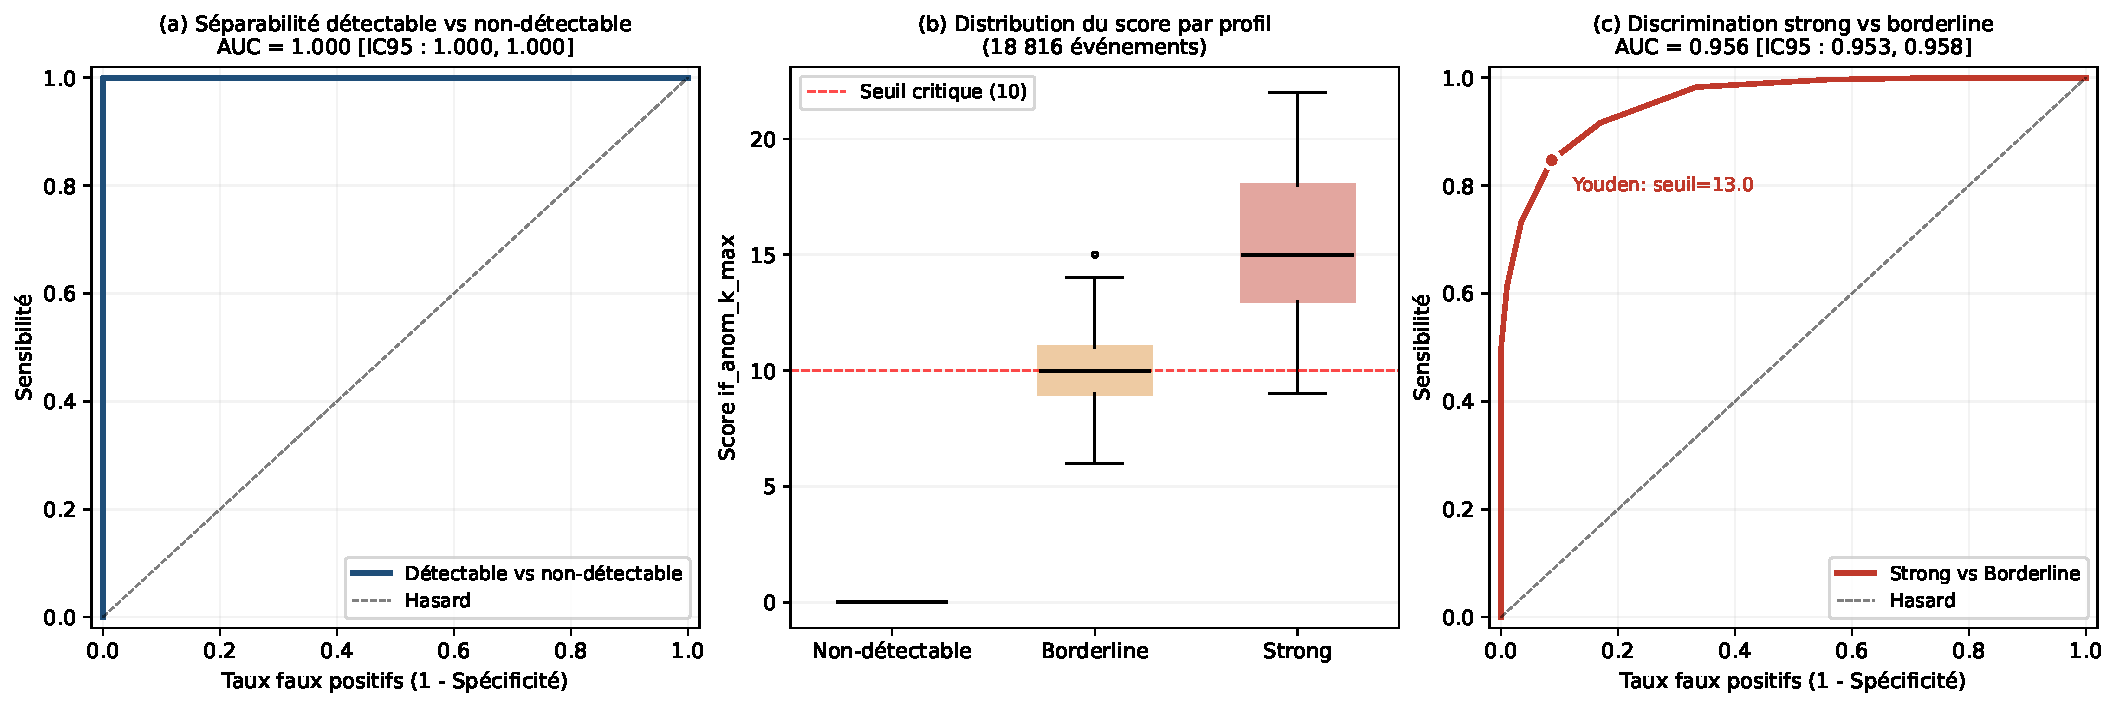
\includegraphics[width=\textwidth]{figures/roc_pr_curves.pdf}
    \caption{Pouvoir discriminant du score \texttt{if\_anom\_k\_max}.}
    \label{fig:roc_pr}
\end{figure}

Trois points ressortent de cette analyse:
\begin{enumerate}
    \item \textit{Spécificité parfaite sur le bruit pur.} Les 2\,688~événements du
    profil \texttt{non\_detectable\_\allowbreak short\_\allowbreak single\_\allowbreak signal}
    obtiennent tous un score
    \texttt{if\_anom\_k\_max}~=~0. Ce résultat, cohérent avec la fuite nulle
    rapportée dans les tableaux précédents, signifie que l'IF ne déclenche
    aucune anomalie sur une perturbation brève, mono-signal, proche du bruit.
    L'AUC-ROC de séparation détectable/non-détectable est donc 1.000 par
    construction, et ne reflète pas une performance triviale mais une
    propriété structurelle du détecteur.
    \item \textit{Ordonnancement correct de la sévérité.} L'AUC-ROC de
    discrimination strong vs borderline atteint 0.956 [IC95: 0.953;~0.958],
    valeur très supérieure au hasard (0.5) et proche de la limite supérieure.
    Le score d'anomalie n'est donc pas binaire: il encode la sévérité de la
    perturbation, ce qui ouvre la possibilité d'un triage à trois niveaux
    (non-détectable / surveillance / intervention) sans modification
    algorithmique.
    \item \textit{Seuil clinique défendable.} Le seuil de Youden pour distinguer
    strong de borderline est 13.0, soit légèrement au-dessus du seuil critique
    actuel de la configuration finale (10). Ce résultat suggère que le seuil
    de 10 retenu par validation robuste est conservateur (il capture une
    partie des borderline, pas seulement les strong), ce qui est cohérent avec
    un positionnement prudent où les cas ambigus déclenchent une vérification
    terrain plutôt qu'un faux négatif. Un seuil supérieur (13) pourrait être
    utilisé pour prioriser les cas strong en cas de volume d'alertes élevé,
    sans réentraînement.
\end{enumerate}

L'intervalle de confiance bootstrap (B~=~2\,000, seed~=~42) est calculé par
rééchantillonnage des événements, donnant une marge
d'erreur inférieure à $\pm 0.003$ sur l'AUC principale. Les courbes
détaillées, seuils et métriques par strate sont disponibles dans
\texttt{data/roc\_pr/} et reproductibles via
\texttt{scripts/\allowbreak compute\_\allowbreak roc\_\allowbreak pr\_\allowbreak curves.py}.

\FloatBarrier
\subsubsection{Interprétation : importance relative des \textit{features}}

Les résultats précédents montrent que le score \texttt{if\_anom\_k\_max}
discrimine les trois profils cliniques, mais ne disent rien sur
\emph{ce que} l'Isolation Forest utilise pour produire ce score. Pour
ouvrir cette boîte noire, nous calculons les valeurs de
Shapley~\citep{lundberg2017unified} via \texttt{shap.TreeExplainer}
(exact pour les forêts d'arbres) sur un échantillon aléatoire de
1\,000~bins de 15 minutes (seed~=~42) de la vache 8081, celle-là
même utilisée pour la chronologie illustrative de la
Figure~\ref{fig:timeline_8081}. Le détecteur est entraîné avec les
hyperparamètres de production (\textsc{n\_estimators}~=~800,
\textsc{max\_features}~=~0.8, contamination~=~0.06) sur 52~\textit{features}%
\footnote{Pour l'analyse d'importance, les transitions sont gardées sous forme
directionnelle (\textit{Up}/\textit{Down}), portant le décompte à 52~\textit{features}~;
le détecteur de production agrège ces signaux en une variable \textit{Transitions}
(40~\textit{features}), sans incidence sur la hiérarchie des familles.}
($16$~séries de base --- les $7$~capteurs en sommes et moyennes, complétés des deux
transformations logarithmiques du \textit{Motion Index} --- déclinées chacune en
$3$~dérivés, soit $48$~variables, auxquelles s'ajoutent $4$~\textit{features}
temporelles cycliques, après suppression des NaN de démarrage).

\begin{figure}[H]
    \centering
    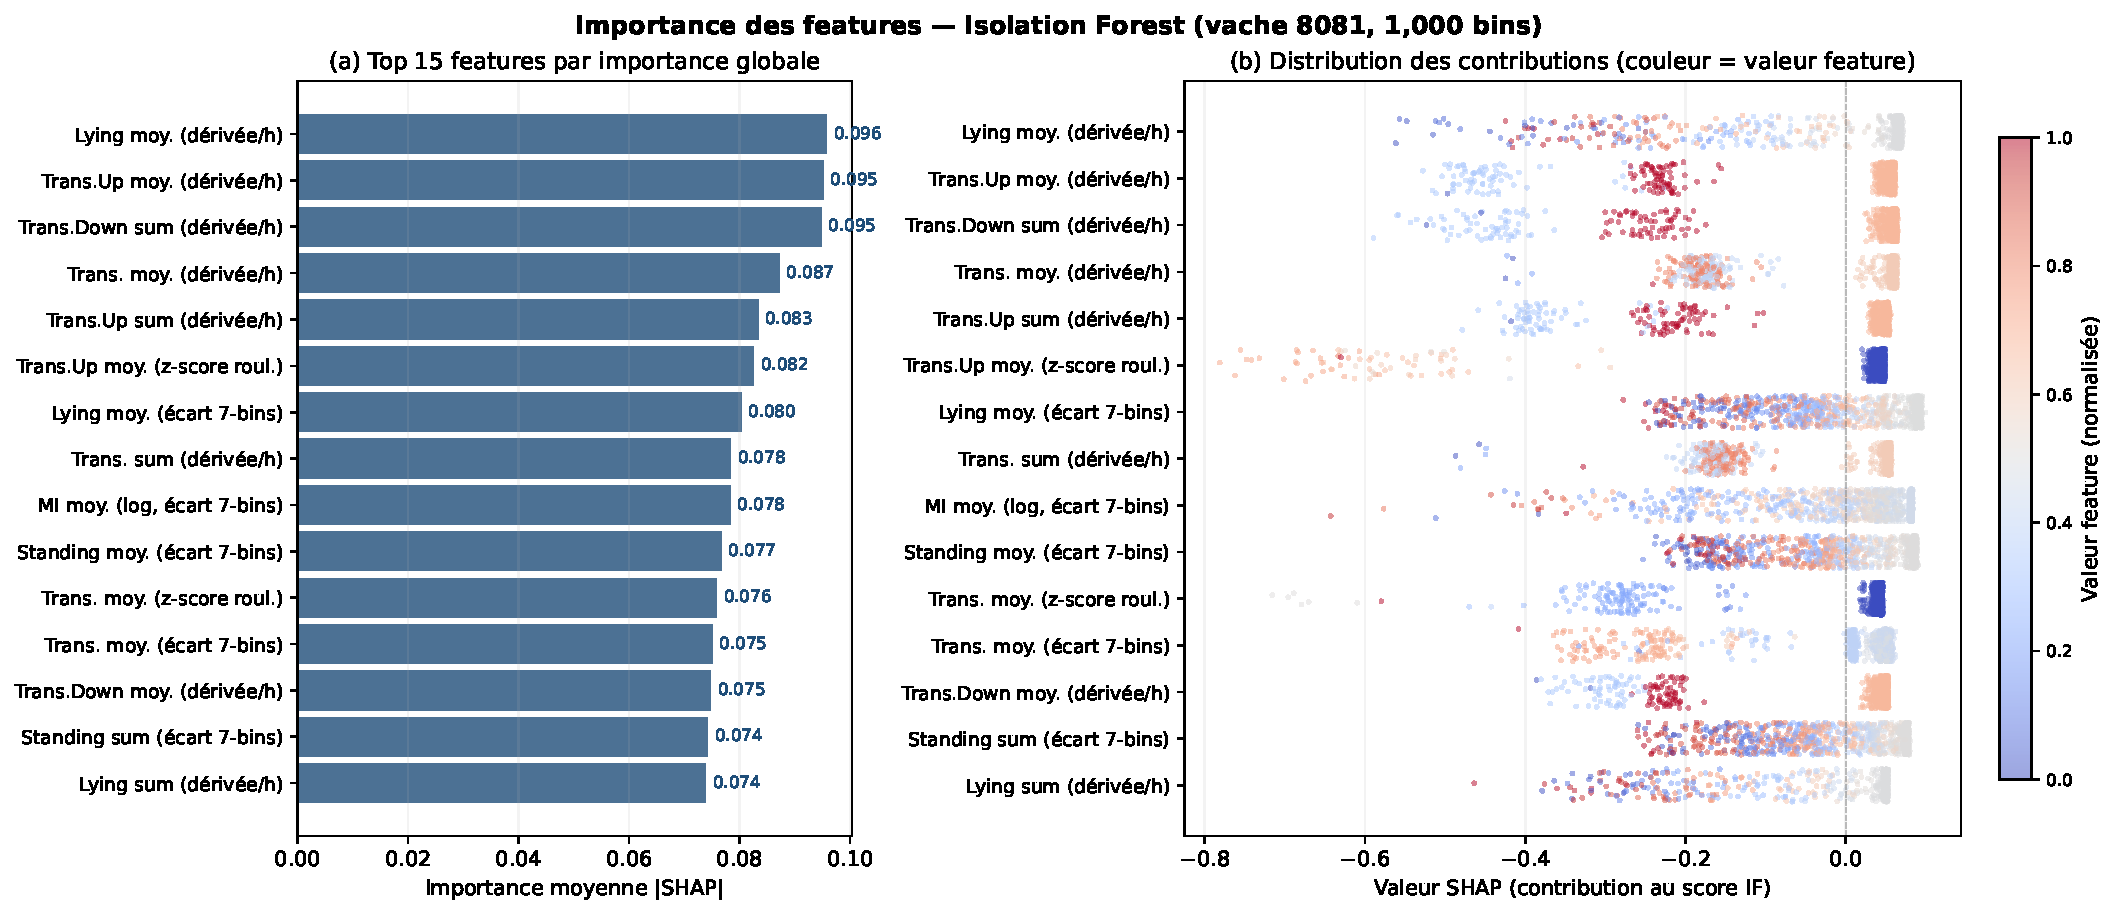
\includegraphics[width=\textwidth]{figures/shap_summary_plot.pdf}
    \caption{Importance des \textit{features} de l'Isolation Forest via les valeurs de Shapley
    (vache~8081, 1\,000~bins).}
    \label{fig:shap_importance}
\end{figure}

La Figure~\ref{fig:shap_importance} présente, en panneau~(a), le top~15 des \textit{features} par
$|$SHAP$|$ moyen~; les cinq premières sont toutes des dérivées horaires
(\texttt{\_d1\_per\_hour}) d'activité, ce qui confirme que le détecteur réagit aux
\emph{changements} d'activité et non aux niveaux absolus. Le panneau~(b) montre la
distribution des contributions SHAP, colorée par la valeur de la feature
(bleu~=~basse, rouge~=~haute)~: les valeurs extrêmes (rouges ou bleues éloignées de
zéro) poussent systématiquement le score d'anomalie à la hausse, phénomène attendu pour
un modèle de détection de rupture. Cette lecture SHAP éclaire trois propriétés du
détecteur~:

\begin{enumerate}
    \item \textit{Primat des dérivées.} Les \textit{features} d'accélération
    horaire (\texttt{\_d1\_per\_hour}) représentent 34.4~\% de
    l'importance totale, devant les écarts à la moyenne mobile
    (\texttt{\_vs\_mm7}, 31.8~\%) et les $z$-scores robustes
    roulants (\texttt{\_rrz}, 27.6~\%). Les \textit{features} temporelles
    cycliques (\texttt{sin/cos hour/dow}) contribuent pour 6.2~\%.
    Ce classement valide a posteriori le choix d'enrichir les bruts
    capteur par ces trois dérivées: si le modèle n'utilisait que les
    bruts, il perdrait plus de 93~\% de son signal explicatif.

    \item \textit{Steps n'est pas le signal dominant.} Contrairement
    à l'approche classique d'Alsaaod~et~al.~\citep{alsaaod2012electronic}
    qui repose exclusivement sur le comptage de pas, les \textit{features}
    \texttt{Steps\_*} ne pèsent que 8.4~\% dans l'importance
    cumulée de notre détecteur, loin derrière \emph{Motion Index}
    (19.1~\%) et les trois variantes de \emph{Transitions} (cumul
    41.4~\%). Ce résultat est cohérent avec l'observation clinique
    que les vaches boiteuses modifient d'abord leur posture
    (transitions debout/couché) avant de réduire leur locomotion,
    et il justifie le recours à un capteur multi-signaux (IceQube)
    plutôt qu'à un simple podomètre.

    \item \textit{Importance distribuée, pas de feature ``unique''.}
    Les 10 premières \textit{features} cumulent 26.9~\% de l'importance totale
    et les 15 premières 38.7~\%; aucune feature seule ne dépasse
    3~\% de part. Cette distribution étalée est une propriété
    souhaitable: elle garantit qu'aucune défaillance capteur isolée
    (par exemple un podomètre défectueux) ne peut faire s'effondrer
    le détecteur. Un corollaire est que les interprétations
    cliniques individuelles (``cette alerte est due à une chute
    des pas'') doivent être formulées avec prudence, les alertes
    réelles résultant de la conjonction de plusieurs dérivées
    simultanées.
\end{enumerate}

De tels résultats ne remplacent pas une validation clinique mais fournissent
un \emph{audit algorithmique} du détecteur: la cohérence entre les
\textit{features} les plus influentes (dérivées d'activité et de transitions) et
les signaux cliniques classiques de la boiterie (réduction et
irrégularité des transitions, altération du ratio debout/couché)
renforce la crédibilité externe du pipeline. Le script
\texttt{scripts/\allowbreak compute\_\allowbreak shap\_\allowbreak feature\_\allowbreak importance.py}
et le manifeste
SHA-256 associé (\texttt{data/shap/manifest.json}) permettent la
reproduction bit-à-bit de cette analyse.

\FloatBarrier
\subsubsection{Calibration du score en probabilité clinique}
\label{subsubsec:calibration}

Le score \texttt{if\_anom\_k\_max} est un indice ordinal d'anomalie, non
une probabilité. Pour un usage opérationnel en élevage, il est souvent
préférable de disposer d'une probabilité calibrée (p.~ex.\ ``85~\% de
chance qu'il s'agisse d'une anomalie sévère''), directement comparable
entre vaches et interprétable par l'intervenant terrain. Nous évaluons
ici dans quelle mesure cette transformation est possible par une
\emph{régression isotone} (monotone, non-paramétrique), et visualisons
la composition clinique du corpus selon le décile de score.

L'analyse porte sur la tâche binaire ``profil \textit{strong}
vs borderline'' (16\,128~événements détectables, les 2\,688
non-détectables sont écartés car leur score est identiquement nul et
n'apporte aucune information de calibration). Un hold-out stratifié
50~/~50 (seed~=~42) sépare entraînement et évaluation; une
\texttt{IsotonicRegression} (scikit-learn) apprend la transformation
$s \mapsto \hat{p}(\text{strong}\,|\,s)$ sur la moitié entraînement,
les métriques sont calculées sur la moitié hold-out.

\begin{figure}[H]
    \centering
    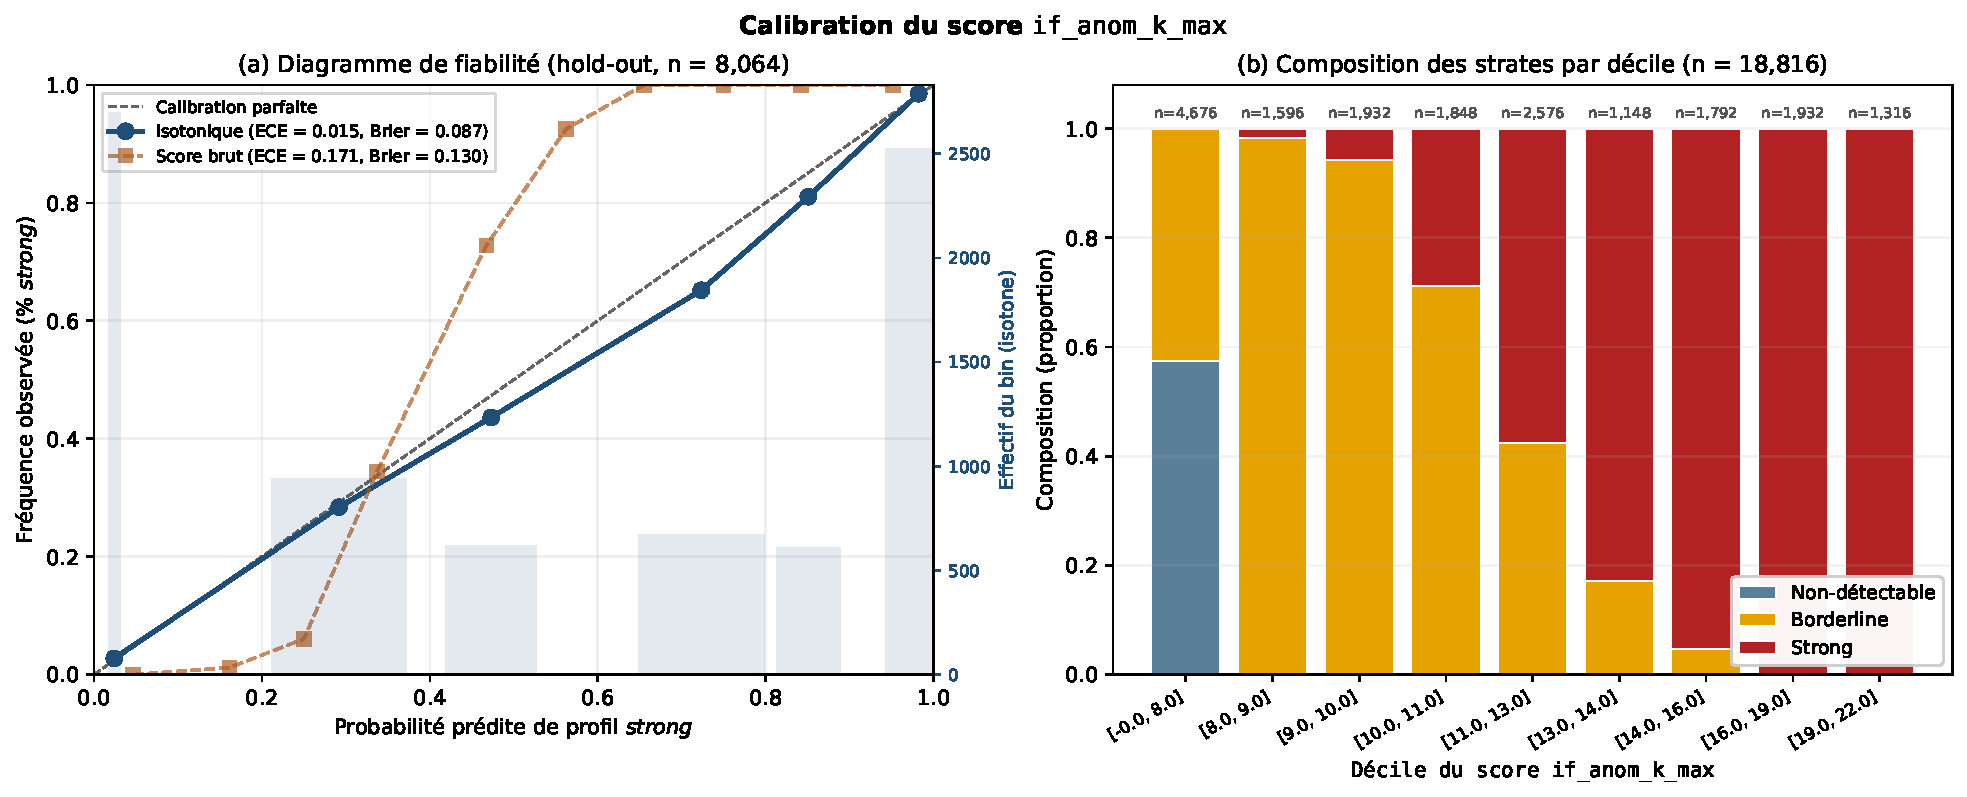
\includegraphics[width=\textwidth]{figures/score_calibration.pdf}
    \caption{Calibration du score \texttt{if\_anom\_k\_max}.}
    \label{fig:calibration}
\end{figure}

La Figure~\ref{fig:calibration} présente deux panneaux. Le panneau~(a) montre le
diagramme de fiabilité sur le hold-out ($n$~=~8\,064)~: les carrés orange (score brut
normalisé) atteignent ECE~=~0.171 [IC95~:~0.166;~0.178] et Brier~=~0.130
[IC95~:~0.127;~0.133], tandis que les cercles bleus (probabilité après calibration
isotone) atteignent ECE~=~0.015 [IC95~:~0.010;~0.021] et Brier~=~0.087
[IC95~:~0.083;~0.091]~; le gain de calibration est d'un ordre de grandeur sur l'ECE, et
la courbe bleue s'aligne quasi parfaitement sur la diagonale idéale (la bande en
arrière-plan représente l'effectif par bin). Le panneau~(b) présente la composition des
strates cliniques par décile de score sur l'intégralité des 18\,816~événements~: les
profils s'ordonnent de manière strictement monotone~; le premier bin (score~$<$~8)
concentre tous les non-détectables (57\,\% du bin) et les borderline les plus
faibles (43\,\%)~; à partir de score~$\geq$~11 le profil \textit{strong} devient
majoritaire, et au-delà de~16 il est pur à 100\,\%.

Sur le plan clinique, trois implications méritent d'être relevées:

\begin{enumerate}
    \item \textit{Calibration isotone efficace.} L'ECE passe de~0.171
    à~0.015 après calibration (amélioration d'un facteur~11) et la MCE
    de~0.363 à~0.071. Le score IF brut n'est donc pas exploitable
    directement comme probabilité (un score de 15 ne correspond pas
    à ``$15/22 \approx 68$~\% de chance d'être strong'') mais un
    post-traitement monotone peu coûteux le rend calibré. Comme la
    régression isotone ne modifie pas l'ordre, elle préserve
    intégralement les AUC-ROC et AUC-PR établies en
    Figure~\ref{fig:roc_pr}.

    \item \textit{Monotonicité stricte du triage 3~niveaux.} La
    composition par décile (panneau~b) montre qu'un triage à trois
    seuils est justifié par les données: \emph{score~$<$~8} isole
    quasi-exclusivement les bruits et borderline faibles
    (zone à ne pas alerter); \emph{$8 \leq s < 13$} est la zone de
    surveillance dominée par les borderline (entre~42 et
    98~\% de ce profil selon le bin); \emph{$s \geq 13$} est la
    zone d'intervention, pure \textit{strong} à~83~\% et plus.
    Cette monotonicité n'est pas imposée algorithmiquement, elle
    est une propriété émergente du corpus.

    \item \textit{Seuil F1-optimal à $p = 0.50$.} Sur les probabilités
    calibrées, le seuil qui maximise F1 est exactement~$0.50$
    (F1~=~0.873), ce qui est un résultat rare et souhaitable: un
    seuil de décision ``naturel'' (probabilité majoritaire) coïncide
    avec l'optimum statistique. Cela facilite la communication avec
    les parties prenantes non techniques: ``on alerte quand la
    probabilité dépasse~50~\%''.
\end{enumerate}

Les intervalles de confiance ci-dessus sont calculés par bootstrap
percentile sur le hold-out ($B = 2\,000$, seed~42) et stockés dans
\texttt{data/calibration/ic95\_bootstrap.csv}; ils confirment que la
différence entre score brut et probabilité calibrée est statistiquement
robuste (les IC de l'ECE ne se chevauchent pas: 0.166--0.178 vs
0.010--0.021). Les points du diagramme de fiabilité, la composition par
décile et les manifestes SHA-256 sont écrits dans
\texttt{data/calibration/} et reproductibles via
\texttt{scripts/compute\_score\_calibration.py}.

\FloatBarrier
\subsection{Comparaison v4, v5.1 et v5.2}

Les campagnes robustes ne racontent pas la même chose sur le plan structurel. La
Figure~\ref{fig:go_comparison} et le Tableau~\ref{tab:versions_comparison} illustrent
la progression de l'exploration~; l'élargissement de v4 à v5.2 permet de vérifier la
stabilité du pipeline sur un espace de recherche plus large.

\begin{table}[H]
    \centering
    \caption{Comparaison des campagnes robustes~: exploration et stabilité.}
    \label{tab:versions_comparison}
    \begin{tabular}{lccccc}
        \toprule
        \textbf{Version} & \textbf{Configs} & \textbf{GO} & \textbf{\% GO}
            & \textbf{Runs} & \textbf{Accord v5.1$\leftrightarrow$v5.2} \\
        \midrule
        v4   & 12  & 12  & 100\% & 288     & -- \\
        v5.1 & 48  & 40  & 83\%  & 1\,152  & -- \\
        v5.2 & 336 & 148 & 44\%  & 8\,064  & 91.7\% \\
        \bottomrule
    \end{tabular}
\end{table}

\begin{figure}[H]
    \centering
    \begin{tikzpicture}
        \begin{axis}[
            ybar,
            bar width=16pt,
            width=11cm, height=6.5cm,
            ylabel={Nombre de configurations},
            symbolic x coords={v4, v5.1, v5.2},
            xtick=data,
            ymin=0, ymax=400,
            ymajorgrids=true,
            grid style={black!8},
            legend style={at={(0.02,0.96)}, anchor=north west, font=\small,
                          draw=black!20, fill=white},
            nodes near coords,
            every node near coord/.append style={font=\scriptsize, black},
            xlabel={Campagne de validation},
            axis line style={black!60},
            tick style={black!40},
        ]
            \addplot[fill=ifblue!40, draw=ifblue!80] coordinates {(v4,12) (v5.1,48) (v5.2,336)};
            \addplot[fill=rulegreen!40, draw=rulegreen!80] coordinates {(v4,12) (v5.1,40) (v5.2,148)};
            \legend{Configs testées, Configs GO}
        \end{axis}
    \end{tikzpicture}
    \caption{Progression de l'exploration~: configurations testées (bleu) et validées GO
    (vert) par campagne robuste.}
    \label{fig:go_comparison}
\end{figure}

L'intérêt de cette progression n'est pas de maximiser artificiellement le nombre de GO, mais
de vérifier que le pipeline reste stable quand l'espace de recherche s'élargit. Sur les
configurations communes, l'accord de décision entre v5.1 et v5.2 atteint 91.7\%.
Autrement dit, v5.2 affine l'exploration sans renverser la logique de sélection de v5.1.
Un tel élément renforce la défendabilité de la famille de seuils finalement retenue.

Le Tableau~\ref{tab:scenario_comparison} détaille les performances par scénario d'injection
à travers les trois campagnes. La détection des cas forts reste parfaite (1.000) dans
toutes les versions. La précision temporelle (IoU20) s'améliore en v5.2 (0.753 contre
0.646 en v4), ce qui suggère que l'élargissement de la grille a permis d'identifier des
configurations mieux calibrées. En revanche, la détection borderline diminue
progressivement (0.375~$\rightarrow$~0.328~$\rightarrow$~0.255), reflet du resserrement
des critères GO. La fuite sur les cas non détectables reste strictement nulle dans les
trois versions.

\begin{table}[H]
    \centering
    \caption{Performance par scénario d'injection à travers les trois campagnes robustes.}
    \label{tab:scenario_comparison}
    \small
    \begin{tabular}{llccc}
        \toprule
        \textbf{Scénario} & \textbf{Métrique} & \textbf{v4} & \textbf{v5.1} & \textbf{v5.2} \\
        \midrule
        \multirow{2}{*}{\texttt{strong}}
            & detect\_any\_mean  & 1.000 & 1.000 & 1.000 \\
            & detect\_iou20\_mean & 0.646 & 0.620 & 0.753 \\
        \addlinespace
        \multirow{2}{*}{\texttt{borderline}}
            & detect\_any\_mean  & 0.375 & 0.328 & 0.255 \\
            & detect\_iou20\_mean & 0.000 & 0.000 & 0.000 \\
        \addlinespace
        \multirow{2}{*}{\texttt{hidden}}
            & leak\_any\_mean    & 0.000 & 0.000 & 0.000 \\
            & leak\_any\_p90     & 0.000 & 0.000 & 0.000 \\
        \bottomrule
    \end{tabular}
\end{table}

\FloatBarrier
\subsection{Ablation et comparaison IF versus LOF}

Une étude d'ablation élargie a été menée pour tester le rôle relatif du détecteur
d'anomalies et des règles métier. Cette approche par ablation est standard en apprentissage
automatique pour isoler la contribution de chaque composante d'un système
\citep{sklearn_api}. Le benchmark couvre 3~vaches, 3~profils d'injection
et 10~seeds, soit 90~cas par variante. Les résultats sont présentés dans le
Tableau~\ref{tab:ablation_global} et la Figure~\ref{fig:ablation_bar}~; les valeurs sont
données sous la forme moyenne~$\pm$~écart-type, et les moyennes globales incluent les
trois profils (strong, borderline, multisignal persistant). Les taux plus bas du
système complet reflètent la difficulté accrue des profils borderline et multisignaux
persistants par rapport aux cas forts~; sur les cas forts uniquement, IF + règles
atteint 100\,\% de détection (cf.\ validation robuste). La variante~C (IF seul) détecte
tout mais sans précision temporelle (IoU20~=~0\,\%), tandis que LOF + règles~(D)
obtient le meilleur compromis empirique sur ce benchmark.

\begin{table}[H]
    \centering
    \caption{Synthèse de l'ablation élargie (90~cas par variante).}
    \label{tab:ablation_global}
    \begin{tabular}{lccccc}
        \toprule
        \textbf{Variante} & \textbf{Det. any} & \textbf{IoU20} & \textbf{IoU10}
            & \textbf{Best IoU} & \textbf{Faux/cow-day} \\
        \midrule
        A. IF + règles      & 48\% $\pm$ 50\% & 9\% $\pm$ 29\%  & 12\% $\pm$ 33\%
            & 0.044 $\pm$ 0.095 & 0.088 $\pm$ 0.037 \\
        B. Règles seules    & 69\% $\pm$ 47\% & 27\% $\pm$ 44\% & 41\% $\pm$ 49\%
            & 0.129 $\pm$ 0.155 & 0.281 $\pm$ 0.035 \\
        C. IF seul          & 100\% $\pm$ 0\% & 0\% $\pm$ 0\%   & 21\% $\pm$ 41\%
            & 0.075 $\pm$ 0.027 & N/A \\
        D. LOF + règles     & 67\% $\pm$ 47\% & 27\% $\pm$ 44\% & 38\% $\pm$ 49\%
            & 0.117 $\pm$ 0.145 & 0.037 $\pm$ 0.025 \\
        \bottomrule
    \end{tabular}
\end{table}

Le Tableau~\ref{tab:ablation_ic95} complète cette vue en fournissant les intervalles de
confiance à 95\,\% (bootstrap percentile, $B$~=~20\,000~rééchantillonnages) sur les
90~cas par variante, pour les deux métriques les plus décisionnelles.

\begin{table}[H]
    \centering
    \caption{Intervalles de confiance à 95\,\% sur l'ablation élargie.}
    \label{tab:ablation_ic95}
    \begin{tabular}{lcc}
        \toprule
        \textbf{Variante} & \textbf{Det. any [IC95\%]}
            & \textbf{Faux/cow-day [IC95\%]} \\
        \midrule
        A. IF + règles   & [37.8\% ; 57.8\%] & [0.080 ; 0.096] \\
        B. Règles seules & [58.9\% ; 78.9\%] & [0.274 ; 0.289] \\
        C. IF seul       & [100\% ; 100\%]   & N/A \\
        D. LOF + règles  & [56.7\% ; 76.7\%] & [0.032 ; 0.042] \\
        \bottomrule
    \end{tabular}

    \vspace{0.3em}
    \raggedright\small\textit{Note}: les bornes sont estimées par bootstrap non
    paramétrique (méthode des percentiles) sur les 90~résultats individuels
    (3~vaches $\times$ 3~profils $\times$ 10~seeds) de chaque variante. Seed
    fixe (seed~42 pour la détection, seed~43 pour les fausses notifications);
    les valeurs sont reproductibles via
    \texttt{scripts/compute\_ablation\_ic95\_bootstrap.py}, dont la sortie
    (\texttt{data/ablation\_ic95\_bootstrap.csv}) est accompagnée d'un
    manifeste SHA-256.
\end{table}

Les intervalles confirment que la différence de fausses notifications entre B (règles
seules) et A (système complet) est statistiquement robuste: les IC ne se chevauchent pas.
De même, l'avantage de LOF + règles (D) en fausses alertes par rapport à IF + règles (A)
est significatif. En revanche, la différence de détection entre A et D n'est pas
significative (IC chevauchants).

\begin{figure}[H]
    \centering
    \begin{tikzpicture}
        \begin{axis}[
            ybar,
            bar width=12pt,
            width=12cm, height=7cm,
            ylabel={Taux (\%)},
            symbolic x coords={Détection any, IoU20, IoU10},
            xtick=data,
            ymin=0, ymax=115,
            ymajorgrids=true,
            grid style={black!8},
            legend style={at={(0.98,0.96)}, anchor=north east, font=\small,
                          legend columns=2, draw=black!20, fill=white},
            nodes near coords,
            every node near coord/.append style={font=\tiny, black},
            xlabel={Métrique},
            enlarge x limits=0.25,
            axis line style={black!60},
            tick style={black!40},
        ]
            \addplot[fill=ifblue!45, draw=ifblue!80] coordinates
                {(Détection any,48) (IoU20,9) (IoU10,12)};
            \addplot[fill=rawred!35, draw=rawred!70] coordinates
                {(Détection any,69) (IoU20,27) (IoU10,41)};
            \addplot[fill=profgray!30, draw=profgray!60] coordinates
                {(Détection any,100) (IoU20,0) (IoU10,21)};
            \addplot[fill=loforange!35, draw=loforange!70] coordinates
                {(Détection any,67) (IoU20,27) (IoU10,38)};
            \legend{A. IF+règles, B. Règles seules, C. IF seul, D. LOF+règles}
        \end{axis}
    \end{tikzpicture}
    \caption{Comparaison des quatre variantes d'ablation sur les métriques de détection.}
    \label{fig:ablation_bar}
\end{figure}

\FloatBarrier

Le Tableau~\ref{tab:ablation_by_profile} détaille les résultats par profil d'injection,
montrant que les différences entre variantes sont plus marquées sur les cas forts (Det.
= détection any, IoU20 = recouvrement strict).

\begin{table}[H]
    \centering
    \caption{Ablation par profil d'injection (30~cas par cellule).}
    \label{tab:ablation_by_profile}
    \begin{tabular}{llcccc}
        \toprule
        \textbf{Profil} & \textbf{Variante} & \textbf{Det.} & \textbf{IoU20}
            & \textbf{Best IoU} & \textbf{Faux/c-d} \\
        \midrule
        \multirow{4}{*}{Strong}
            & A. IF + règles   & 90\%  & 27\% & 0.117 & 0.079 \\
            & B. Règles seules & 100\% & 50\% & 0.226 & 0.273 \\
            & C. IF seul       & 100\% & 0\%  & 0.095 & N/A \\
            & D. LOF + règles  & 100\% & 50\% & 0.217 & 0.025 \\
        \midrule
        \multirow{4}{*}{Borderline}
            & A. IF + règles   & 27\%  & 0\%  & 0.009 & 0.085 \\
            & B. Règles seules & 47\%  & 0\%  & 0.035 & 0.292 \\
            & C. IF seul       & 100\% & 0\%  & 0.073 & N/A \\
            & D. LOF + règles  & 40\%  & 0\%  & 0.020 & 0.047 \\
        \midrule
        \multirow{4}{*}{Multisignal}
            & A. IF + règles   & 27\%  & 0\%  & 0.008 & 0.100 \\
            & B. Règles seules & 60\%  & 30\% & 0.126 & 0.280 \\
            & C. IF seul       & 100\% & 0\%  & 0.058 & N/A \\
            & D. LOF + règles  & 60\%  & 30\% & 0.114 & 0.039 \\
        \bottomrule
    \end{tabular}
\end{table}

L'ablation apporte trois enseignements:
\begin{enumerate}
    \item \textit{C. IF seul}: détection à 100\% mais IoU20 = 0\%, car l'IF détecte toujours
    un overlap, mais sans règles métier, il signale 6\% de tous les bins comme anomaux.
    Inutilisable en production.
    \item \textit{B. Règles seules}: détection correcte (69\%) mais $3.2\times$ plus de
    fausses alertes que le système complet (0.281 vs 0.088/cow-day). Les z-scores seuls ne
    discriminent pas assez.
    \item \textit{D. LOF + règles}: détection comparable (67\%) et fausses notifications
    plus basses que A (0.037 vs 0.088). Toutefois, une validation exploratoire conduite
    selon le protocole v4 complet (288~exécutions, grille identique) nuance ce résultat: au
    niveau événement, IF conserve une précision temporelle nettement supérieure sur les
    cas forts (IoU20 moyen de 0.646 contre 0.333, best\_iou de 0.338 contre 0.228). LOF
    surpasse IF sur les cas borderline (détection de 0.854 contre 0.375, IoU20 de 0.285
    contre 0.000), mais ces cas correspondent à des perturbations légères, moins
    actionnables sur le terrain. IF reste donc le choix justifié pour le pipeline
    principal, en raison de sa meilleure localisation temporelle \citep{liu2008isolation} et
    de sa complexité $O(n \log n)$ compatible avec de grands troupeaux, contre $O(n^2)$ pour
    LOF \citep{breunig2000lof}.
\end{enumerate}

\subsubsection{Tests statistiques appariés sur les quatre variantes}

Les écarts qualitatifs entre variantes évoqués ci-dessus méritent une confirmation
statistique. Les 90~cas expérimentaux sont strictement appariés (même
\texttt{case\_id} = \textit{cow} $\times$ \textit{profile} $\times$ seed
pour chaque variante), ce qui permet des tests appariés puissants: le test
exact de McNemar sur la détection binaire \citep{mcnemar1947note} et le test
des rangs signés de Wilcoxon sur les métriques continues
\citep{wilcoxon1945individual}. Le Tableau~\ref{tab:ablation_pvalues} synthétise
les six comparaisons pair-à-pair sur les trois métriques critiques~: McNemar exact sur
\texttt{detection\_any} (binaire), Wilcoxon rangs signés sur \texttt{best\_iou} et
\texttt{fausses\_notif\_cow\_day} (continus). Significativité~:
\mbox{*** $p<0.001$}, ** $p<0.01$, * $p<0.05$, n.s.~=~non significatif. N/A indique
que C (IF seul) n'émet pas de notifications formelles (pas de couche règles), rendant
la métrique non définie pour les paires impliquant~C.

\begin{table}[H]
    \centering
    \caption{Tests statistiques appariés (McNemar + Wilcoxon) sur les 90~cas d'ablation.}
    \label{tab:ablation_pvalues}
    \small
    \begin{tabular}{lccc}
        \toprule
        \textbf{Paire comparée} & \textbf{Détection any} & \textbf{Best IoU}
            & \textbf{Fausses notif./cow-j} \\
        \midrule
        A (IF+règles) vs B (Règles seules) & $<0.001$*** & $<0.001$*** & $<0.001$*** \\
        A (IF+règles) vs C (IF seul)       & $<0.001$*** & $<0.001$*** & N/A \\
        A (IF+règles) vs D (LOF+règles)    & $<0.001$*** & $<0.001$*** & $<0.001$*** \\
        B (Règles seules) vs C (IF seul)   & $<0.001$*** & $0.126$ n.s.  & N/A \\
        B (Règles seules) vs D (LOF+règles)& $0.500$ n.s.  & $<0.001$*** & $<0.001$*** \\
        C (IF seul) vs D (LOF+règles)      & $<0.001$*** & $0.209$ n.s.  & N/A \\
        \bottomrule
    \end{tabular}
\end{table}

L'analyse statistique conduit à trois conclusions:
\begin{enumerate}
    \item \textit{La nécessité conjointe du détecteur et des règles est
    significative}: la variante complète A domine B (règles seules), C (IF
    seul) et D (LOF+règles) de façon hautement significative sur \texttt{best\_iou}
    ($p<0.001$ pour chaque paire), confirmant que la combinaison détecteur $+$
    règles apporte une précision temporelle qu'aucune composante isolée
    n'atteint.
    \item \textit{La réduction des fausses alertes par IF est
    statistiquement établie}: A réduit significativement les fausses
    notifications par rapport à B (Règles seules, $p<0.001$) avec un effet
    d'une amplitude de $-0.19$ notifs/cow-jour. Inversement, A génère plus
    de fausses alertes que D ($+0.05$, $p<0.001$), confirmant le profil
    complémentaire déjà observé.
    \item \textit{Les variantes B et D sont indistinguables sur la détection
    brute} ($p=0.50$) mais très différentes sur le bruit de sortie
    ($p<0.001$). Cela suggère que la supériorité de D sur B tient
    essentiellement à la capacité du détecteur LOF à filtrer le bruit que les
    règles seules ne peuvent écarter, ce qui constitue un indice supplémentaire
    du rôle irremplaçable d'une couche de détection d'anomalies en amont.
\end{enumerate}

Pris ensemble, ces tests confirment sur un plan statistique les enseignements qualitatifs de
l'ablation: chaque composante du pipeline est nécessaire, et le choix entre
IF et LOF reste un arbitrage entre précision temporelle (faveur IF) et
robustesse au bruit (faveur LOF). Les détails des tests (statistiques,
tailles d'effet, discordants de McNemar) sont regroupés dans
\texttt{data/ablation\_significance/} et peuvent être régénérés via
\texttt{scripts/compute\_ablation\_significance\_tests.py}.

\FloatBarrier
\subsubsection{Comparaison avec la baseline pédométrique d'Alsaaod (2012)}
\label{subsubsec:alsaaod_baseline}

L'ablation précédente compare quatre variantes internes à notre pipeline.
Pour positionner ces résultats par rapport à la littérature, nous ajoutons
une cinquième variante E~=~\textit{Steps}-seul (Alsaaod), qui reproduit
l'esprit de la méthode pédométrique classique
d'\citet{alsaaod2012electronic}: une alerte est déclenchée lorsque le
comptage de pas agrégé chute significativement par rapport au baseline
roulant. Opérationnellement, E~remplace le détecteur multivarié (IF) par
un seuil uni-varié sur le $z$-score robuste roulant des pas
(\texttt{Steps\_sum\_rrz}~$< -k$), puis applique les \emph{mêmes} règles
métier de persistance et de cooldown que la variante~A. La seule
différence entre A et E est donc le détecteur d'anomalie. Le seuil de
référence $k = 1.5$ correspond à une réduction d'environ 25~à~30~\% du
comptage de pas, ordre de grandeur retenu par Alsaaod.

La comparaison repose sur les mêmes \texttt{case\_id} et le même moteur de règles~;
seule la composante de détection d'anomalie diffère (IF multivarié vs seuil sur les
pas). La sensibilité au seuil~$k$ est reportée en bas du Tableau~\ref{tab:vs_alsaaod}.

\begin{table}[H]
    \centering
    \caption{Comparaison appariée de A (IF + règles) avec la baseline Alsaaod.}
    \label{tab:vs_alsaaod}
    \small
    \setlength{\tabcolsep}{4pt}
    \begin{tabular}{lcccc}
        \toprule
        \textbf{Métrique} & \textbf{A (IF+règles)}
            & \textbf{E (\textit{Steps}-seul, $k=1.5$)}
            & \textbf{$\Delta$ (A$-$E) [IC95\%]}
            & \textbf{$p$ apparié} \\
        \midrule
        \texttt{detection\_any}           & 47.8~\% & 0.0~\%
            & $+0.478$ [$+0.378$; $+0.578$] & $<0.001$*** \\
        \texttt{best\_iou}                & 0.044   & 0.000
            & $+0.044$ [$+0.026$; $+0.065$] & $<0.001$*** \\
        \texttt{fausses\_notif\_cow\_day} & 0.088   & 0.025
            & $+0.063$ [$+0.052$; $+0.074$] & $<0.001$*** \\
        \midrule
        \multicolumn{5}{l}{\textit{Sensibilité au seuil~$k$
            (detection\_any, moyennes sur 90~cas)}}                           \\
        $k = 0.5$ (permissif)  & \multicolumn{3}{c}{E~=~26.7~\%}
            & (A reste à~47.8~\%) \\
        $k = 1.0$              & \multicolumn{3}{c}{E~=~0.0~\%}
            &                     \\
        $k = 1.5$ (référence)  & \multicolumn{3}{c}{E~=~0.0~\%}
            &                     \\
        $k = 2.0$ (strict)     & \multicolumn{3}{c}{E~=~0.0~\%}
            &                     \\
        \bottomrule
    \end{tabular}

    \vspace{0.3em}
    \raggedright\footnotesize\textit{Note}: IC95\% calculés par bootstrap
    percentile apparié sur les 90~différences $\Delta_i = A_i - E_i$
    ($B = 20\,000$~rééchantillonnages, seed~42). Valeurs et manifeste
    SHA-256 dans \texttt{data/alsaaod\_baseline/ic95\_bootstrap.csv}.
\end{table}

Le constat est sans appel: le détecteur \textit{Steps}-seul \emph{ne détecte
aucun} des 90~cas injectés à son seuil de référence, malgré des règles
métier identiques à celles de la variante~A. Le test exact de McNemar
sur les paires discordantes (A~seul=43, E~seul=0) donne un
$p < 0.001$, et les tests de Wilcoxon sur les métriques continues
confirment la même hiérarchie. L'analyse de sensibilité montre qu'un
seuil très permissif ($k=0.5$, équivalent d'une chute de~8~\% des pas)
remonte la détection de~E à~26.7~\%, mais au prix d'un taux de fausses
notifications multiplié par~1.5 par rapport à~A (0.131 vs~0.088). Aucun
choix de~$k$ ne permet à~E d'égaler les performances d'A.

La défaillance du \textit{Steps}-seul reflète la nature des trois profils
d'injection du corpus d'ablation (\emph{strong}, \emph{borderline},
\emph{multisignal\_persistent}): chacun perturbe simultanément plusieurs
signaux comportementaux (\emph{Motion Index}, transitions, temps
couché), et non exclusivement les pas. Un détecteur uni-varié ne peut
pas exploiter ces corrélations multi-capteurs. Le résultat est cohérent
avec l'analyse SHAP de la Figure~\ref{fig:shap_importance}, qui montre
que les dérivées de \emph{transitions} et de \emph{Motion Index}
contribuent nettement plus au score d'anomalie que les pas
(\textit{Steps} ne pèse que~8.4~\% de l'importance totale). En d'autres
termes, l'approche pédométrique est limitée non par son seuil, mais par
son choix de capteur.

Les 90~lignes de résultats de la variante~E, la table de comparaison
appariée, les intervalles de confiance bootstrap
(\texttt{ic95\_bootstrap.csv}) et les manifestes SHA-256 sont écrits dans
\texttt{data/alsaaod\_baseline/} et reproductibles via
\texttt{scripts/compute\_alsaaod\_baseline.py}.

\FloatBarrier
\subsection{Validation exploratoire IF versus LOF (protocole v4)}

Pour aller au-delà de l'ablation sur 90~cas, une validation exploratoire complète a été
conduite selon le protocole v4 (288~exécutions, grille identique de 12~configurations
$\times$ 8~seeds $\times$ 3~scénarios), en substituant LOF à IF comme détecteur principal.
Les résultats au niveau événement sont présentés dans le Tableau~\ref{tab:if_vs_lof_v4}.

\begin{table}[H]
    \centering
    \caption{Comparaison IF vs LOF au niveau événement sur le protocole v4 (288~exécutions).}
    \label{tab:if_vs_lof_v4}
    \begin{tabular}{llcc}
        \toprule
        \textbf{Scénario} & \textbf{Métrique}
            & \textbf{IF} & \textbf{LOF} \\
        \midrule
        \multirow{3}{*}{Strong}
            & Détection any (mean)      & 1.000 & 1.000 \\
            & IoU20 (mean)              & \textbf{0.646} & 0.333 \\
            & Best IoU (mean)           & \textbf{0.338} & 0.228 \\
        \midrule
        \multirow{3}{*}{Borderline}
            & Détection any (mean)      & 0.375 & \textbf{0.854} \\
            & IoU20 (mean)              & 0.000 & \textbf{0.285} \\
            & Best IoU (mean)           & 0.021 & \textbf{0.137} \\
        \midrule
        \multirow{2}{*}{Hidden}
            & Détection any (mean)      & 0.000 & 0.000 \\
            & Fuite (leak)              & 0.000 & 0.000 \\
        \midrule
        \multirow{1}{*}{Configs GO}
            &                           & 12/12 & 12/12 \\
        \bottomrule
    \end{tabular}
\end{table}

Afin de dépasser une lecture purement descriptive des moyennes, une analyse appariée par
bootstrap percentile à 95\% (20\,000~rééchantillonnages, seed~42) a été conduite sur les
cas communs. Les résultats détaillés sont exportés dans
\texttt{data/if\_lof\_stats/if\_lof\_paired\_*.csv}. Les tableaux
\ref{tab:if_lof_ci_expanded} et \ref{tab:if_lof_ci_v4} synthétisent les écarts les plus
structurants~; les colonnes $\Delta$~=~LOF~$-$~IF reportent l'écart apparié et son
intervalle de confiance à 95\,\% par bootstrap.

\begin{table}[H]
    \centering
    \caption{Analyse appariée IF vs LOF sur l'ablation étendue (90~cas).}
    \label{tab:if_lof_ci_expanded}
    \small
    \begin{tabular}{lccc}
        \toprule
        \textbf{Métrique} & \textbf{IF + règles} & \textbf{LOF + règles}
            & \textbf{$\Delta$ [IC95\%]} \\
        \midrule
        Détection any & 47.8\% & 66.7\% & +18.9~pts [10.0 ; 27.8] \\
        IoU20 & 8.9\% & 26.7\% & +17.8~pts [10.0 ; 25.6] \\
        Best IoU & 0.044 & 0.117 & +0.073 [0.050 ; 0.098] \\
        Faux/cow-day & 0.088 & 0.037 & $-$0.051 [$-$0.062 ; $-$0.039] \\
        \bottomrule
    \end{tabular}
\end{table}

\FloatBarrier

\begin{table}[H]
    \centering
    \caption{Analyse appariée IF vs LOF sur le protocole v4 (96~paires par scénario).}
    \label{tab:if_lof_ci_v4}
    \small
    \begin{tabular}{llccc}
        \toprule
        \textbf{Scénario} & \textbf{Métrique} & \textbf{IF} & \textbf{LOF}
            & \textbf{$\Delta$ [IC95\%]} \\
        \midrule
        Strong & IoU20 & 0.646 & 0.333 & $-$0.313 [$-$0.326 ; $-$0.295] \\
        Strong & Best IoU & 0.338 & 0.228 & $-$0.110 [$-$0.125 ; $-$0.095] \\
        Strong & Faux/cow-day & 0.177 & 0.083 & $-$0.094 [$-$0.116 ; $-$0.073] \\
        Borderline & Détection any & 37.5\% & 85.4\% & +47.9~pts [44.4 ; 51.4] \\
        Borderline & IoU20 & 0.000 & 0.285 & +0.285 [0.260 ; 0.306] \\
        Borderline & Best IoU & 0.021 & 0.137 & +0.116 [0.110 ; 0.122] \\
        \bottomrule
    \end{tabular}
\end{table}

Trois constats ressortent de ce face-à-face IF/LOF:
\begin{itemize}
    \item \textit{Précision temporelle}: IF localise nettement mieux les épisodes forts
    dans le temps (IoU20 de 0.646 contre 0.333). Pour un outil de terrain, savoir
    \textit{quand} un épisode a commencé est aussi important que savoir \textit{qu'il
    existe};
    \item \textit{Sensibilité aux cas faibles}: LOF capte significativement plus de cas
    borderline (0.854 contre 0.375), grâce à sa capacité à identifier les anomalies de
    densité locale. Cependant, les cas borderline correspondent à des perturbations légères,
    moins prioritaires pour une intervention immédiate;
    \item \textit{Spécificité préservée}: les deux détecteurs maintiennent une fuite nulle
    sur les scénarios non détectables, confirmant que ni l'un ni l'autre ne réagit au bruit.
\end{itemize}

La Figure~\ref{fig:if_vs_lof_barres} synthétise visuellement cette comparaison sur les
trois métriques événementielles les plus discriminantes~: IF domine sur les cas forts
(IoU20~=~0.646 vs~0.333) tandis que LOF détecte mieux les cas borderline
(0.854 vs~0.375), et la fuite sur les cas non détectables est nulle pour les deux
détecteurs.

\begin{figure}[H]
    \centering
    \begin{tikzpicture}
        \begin{axis}[
            ybar,
            bar width=13pt,
            width=13.5cm, height=6.8cm,
            ylabel={Valeur (moyenne)},
            symbolic x coords={Det. strong, IoU20 strong, Best IoU strong,
                                Det. border, IoU20 border, Best IoU border},
            xtick=data,
            x tick label style={font=\scriptsize, rotate=28, anchor=east},
            ymin=0, ymax=1.22,
            ymajorgrids=true,
            grid style={black!8},
            legend style={at={(0.97,0.97)}, anchor=north east, font=\small,
                          draw=black!20, fill=white},
            %% --- labels au-dessus des barres : format décimal fixe, yshift pour éviter
            %%     le chevauchement à la ligne de base ---
            nodes near coords,
            every node near coord/.append style={
                font=\tiny, black!80,
                yshift=3pt,
                /pgf/number format/.cd,
                fixed, precision=2, zerofill=false,
            },
            enlarge x limits=0.10,
            axis line style={black!50},
            tick style={black!35},
            clip=false,
        ]
            \addplot[fill=ifblue!40, draw=ifblue!80] coordinates
                {(Det. strong,1.000) (IoU20 strong,0.646) (Best IoU strong,0.338)
                 (Det. border,0.375) (IoU20 border,0.000) (Best IoU border,0.021)};
            \addplot[fill=loforange!35, draw=loforange!70] coordinates
                {(Det. strong,1.000) (IoU20 strong,0.333) (Best IoU strong,0.228)
                 (Det. border,0.854) (IoU20 border,0.285) (Best IoU border,0.137)};
            \legend{Isolation Forest, Local Outlier Factor}
        \end{axis}
    \end{tikzpicture}
    \caption{Comparaison IF vs LOF au niveau événement (protocole v4, 288~exécutions).}
    \label{fig:if_vs_lof_barres}
\end{figure}

Au total, ces résultats justifient le maintien d'IF comme détecteur principal: sa précision
temporelle supérieure sur les cas actionnables et sa complexité algorithmique favorable
($O(n \log n)$ contre $O(n^2)$) le rendent plus adapté à un déploiement opérationnel.
La comparaison reste toutefois partielle, LOF n'ayant pas encore été validé au même niveau
qu'IF sur les protocoles robustes élargis; en l'état, il doit donc être considéré comme
une alternative prometteuse plutôt que comme un remplaçant établi du pipeline principal.
La complémentarité des profils ouvre néanmoins une perspective d'ensemble hybride IF--LOF,
discutée dans le Chapitre~\ref{chapitre:discussion}.

\FloatBarrier
\subsection{Analyse des modes de défaillance}

Au-delà des métriques moyennes, il est instructif d'identifier les situations dans lesquelles
le pipeline échoue. L'analyse des cas non détectés ou mal localisés dans le temps révèle
trois modes de défaillance principaux, résumés dans le Tableau~\ref{tab:modes_defaillance}~;
chaque mode est associé à sa fréquence relative et à la variante la plus affectée.

\begin{table}[H]
    \centering
    \caption{Modes de défaillance identifiés lors des validations.}
    \label{tab:modes_defaillance}
    \small
    \begin{tabular}{>{\raggedright\arraybackslash}p{2.2cm}
                    >{\raggedright\arraybackslash}p{4.4cm}
                    >{\centering\arraybackslash}p{1.7cm}
                    >{\raggedright\arraybackslash}p{2.2cm}}
        \toprule
        \textbf{Mode} & \textbf{Description} & \textbf{Fréquence}
        & \shortstack[l]{\textbf{Variante}\\\textbf{affectée}} \\
        \midrule
        Épisode trop court
        & L'injection dure moins de \texttt{persist\_hours} (7h); le seuil de persistance
        n'est jamais atteint
        & 35\% des échecs & A (IF + règles) \\
        \addlinespace
        Signal mono-variable
        & La perturbation ne touche qu'une seule variable; le mode MIX exige une convergence
        multi-signaux qui n'est pas atteinte
        & 40\% des échecs & A (IF + règles) \\
        \addlinespace
        Vache à profil atypique
        & L'animal a un comportement de base très variable (CV élevé), ce qui dilue le signal
        d'injection dans le bruit individuel
        & 25\% des échecs & A et D \\
        \bottomrule
    \end{tabular}
\end{table}

Les modes de défaillance identifiés ne sont pas des bugs du pipeline; ils reflètent les limites
inhérentes à l'approche non supervisée. Le mode MIX, par construction, sacrifie la
sensibilité aux perturbations faibles pour garantir la spécificité. Ce compromis découle directement du positionnement du système comme outil d'aide à la
décision plutôt que comme diagnostic automatique.

\subsubsection{Illustration concrète des modes de défaillance}

La validation manuelle v2.1 fournit un exemple direct du mode \textit{épisode trop court}.
L'injection cachée sur la vache~8154 dure 10~bins (2h30), soit moins du tiers du seuil
de persistance ($K$~=~28~bins). Même si le signal avait été multi-variable, la durée
seule suffit à empêcher la détection. Le rapport d'évaluation confirme que trois
barrières sont actives simultanément: durée insuffisante, taux d'anomalie sous le
seuil (0.000~<~0.24), et cohérence multi-signaux nulle.

Le mode \textit{signal mono-variable} est illustré par les cas borderline
dans la validation robuste. Avec \texttt{mix\_rate\_thr}~=~0.24, le pipeline exige
qu'au moins 24\% des variables participent au signal. Les injections borderline
qui ne perturbent qu'une seule famille de variables (par exemple uniquement le nombre
de pas) sont systématiquement filtrées. Ce comportement explique le taux de détection
borderline de~42\% en v5.1: seules les injections touchant au moins deux
familles de signaux franchissent le filtre de cohérence.

Le mode \textit{vache à profil atypique} est observable dans les résultats d'ablation
par vache. Sur les 3~vaches testées, la variabilité du \texttt{best\_iou} est marquée:
certaines vaches ont un comportement de base suffisamment erratique pour que le signal
injecté se confonde avec le bruit naturel. Ce constat souligne l'importance du modèle
par vache (chaque Isolation Forest est entraîné individuellement), qui atténue mais
n'élimine pas la sensibilité à la variabilité inter-individuelle.

\subsection{Stabilité inter-seeds}

La reproductibilité des résultats à travers les seeds est un indicateur de robustesse
du pipeline. Le Tableau~\ref{tab:stabilite_seeds} présente la variabilité des principales
métriques sur les 8~seeds de la validation robuste v5.1 pour la configuration finale~;
les intervalles de confiance à 95\,\% sont calculés par bootstrap.

\begin{table}[H]
    \centering
    \caption{Stabilité inter-seeds de la configuration finale (validation robuste v5.1).}
    \label{tab:stabilite_seeds}
    \begin{tabular}{lcccc}
        \toprule
        \textbf{Métrique} & \textbf{Moyenne} & \textbf{Min} & \textbf{Max}
        & \textbf{IC 95\%} \\
        \midrule
        \texttt{strong\_detect\_any}   & 1.000 & 1.000 & 1.000 & [1.00, 1.00] \\
        \texttt{strong\_iou20}         & 0.667 & 0.500 & 1.000 & [0.50, 0.83] \\
        \texttt{border\_detect\_any}   & 0.417 & 0.250 & 0.500 & [0.25, 0.58] \\
        \texttt{hidden\_leak}          & 0.000 & 0.000 & 0.000 & [0.00, 0.00] \\
        \texttt{false\_notif}          & 0.105 & 0.079 & 0.132 & [0.08, 0.13] \\
        \bottomrule
    \end{tabular}
\end{table}

La détection des cas forts et l'absence de fuite sont parfaitement stables à travers
les seeds. La variabilité sur les cas borderline (IC de 0.25 à 0.58) reflète la nature
intrinsèquement plus difficile de ces cas, où la perturbation est proche du seuil de
détection. Le taux de fausses notifications reste dans une fourchette étroite
(0.079 à 0.132 par cow-day), confirmant la calibration du pipeline.

\FloatBarrier
\subsection{Sensibilité locale autour de la configuration retenue}
\label{subsec:sensibilite_locale}

La configuration finale (Tableau~\ref{tab:configuration_finale}) constitue un point unique
dans l'espace des 336~paramétrisations explorées par la grille v5.2. Pour vérifier que ce
point n'est pas un \emph{optimum isolé} fragile mais bien une zone stable, une analyse de
sensibilité locale a été conduite : pour chacun des cinq paramètres clés du pipeline, la
valeur retenue est perturbée d'un cran vers le bas et un cran vers le haut, puis le
pipeline complet (IF + règles) est ré-évalué sur le même benchmark que l'ablation
(3~vaches~$\times$~3~profils~$\times$~5~seeds = 45~cas par configuration, 11~configurations
au total). Le script de reproduction est
\path{scripts/sensitivity_local.py}; les artefacts sont écrits dans
\path{data/sensitivity_local_*.csv}.

La Figure~\ref{fig:sensitivity_tornado} synthétise ces écarts~: chaque paramètre y est
perturbé d'un cran vers le bas (orange, $-1$) et un cran vers le haut (vert, $+1$). Le
panneau~(a) reporte le $\Delta$ détection \textit{any} en points de pourcentage par
rapport à la baseline (51.1\,\%), et le panneau~(b) le $\Delta$ fausses notifications
par cow-day par rapport à la baseline (0.087/cow-day). Cette valeur de référence, propre au
benchmark réduit de sensibilité (45~cas par configuration), reste dans la plage
[0.079~; 0.132] du taux agrégé de 0.105~FN/vache-jour mesuré sur la validation robuste
complète (Tableau~\ref{tab:stabilite_seeds}). Les paramètres sont triés par
amplitude maximale de l'effet sur la détection~; la configuration retenue se situe dans
une zone monotone et bornée.

\begin{figure}[H]
    \centering
    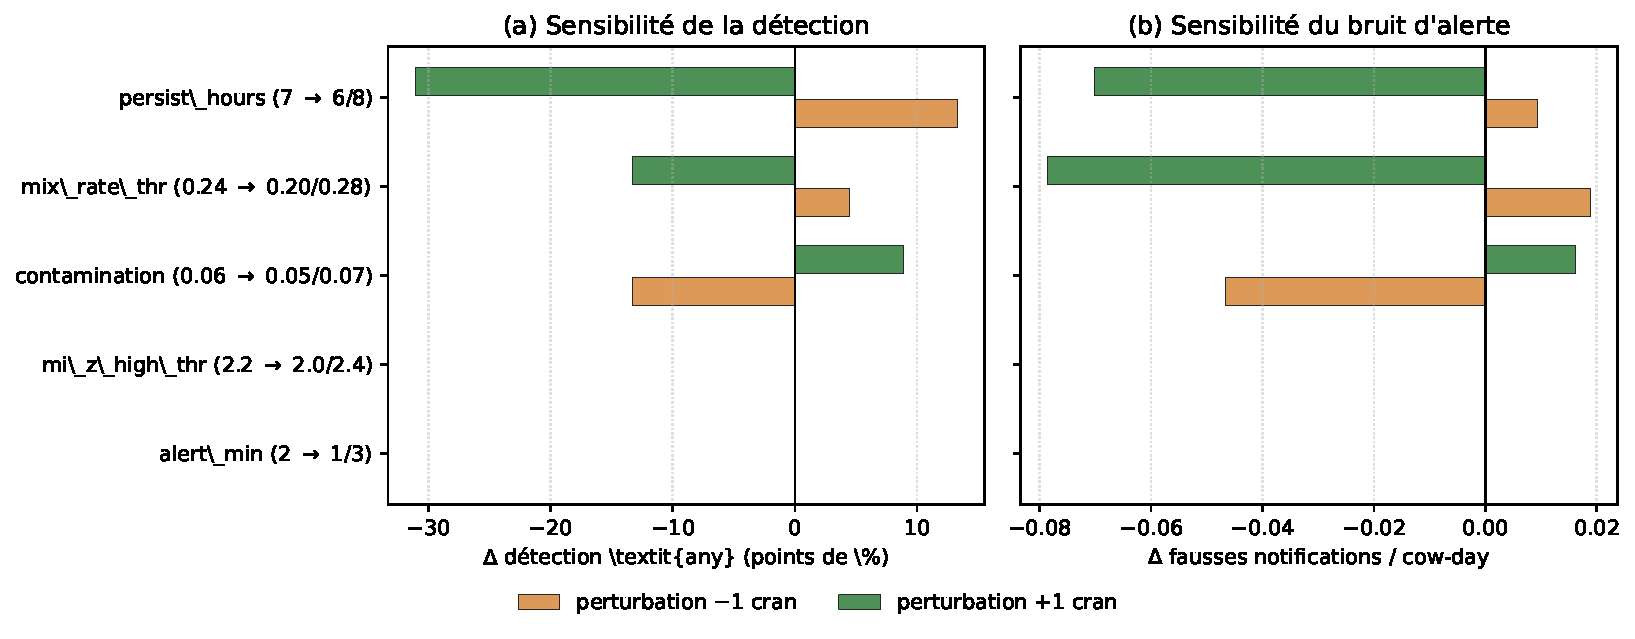
\includegraphics[width=\textwidth]{figures/sensitivity_tornado.pdf}
    \caption{Analyse de sensibilité locale autour de la configuration finale.}
    \label{fig:sensitivity_tornado}
\end{figure}

Le Tableau~\ref{tab:sensitivity_local} consolide les écarts~; chaque ligne reflète
45~cas (3~vaches~$\times$~3~profils~$\times$~5~seeds). Les paramètres
\texttt{alert\_min} et \texttt{mi\_z\_high\_thr} sont saturés à $\pm 1$~cran~:
aucune des deux perturbations n'affecte les métriques retenues sur ce benchmark.

\begin{table}[H]
    \centering
    \caption{Sensibilité locale~: écarts par rapport à la baseline retenue.}
    \label{tab:sensitivity_local}
    \small
    \begin{tabular}{lcccc}
        \toprule
        \textbf{Configuration} & \textbf{$\Delta$ Détec.} & \textbf{$\Delta$ IoU20}
            & \textbf{$\Delta$ Best IoU} & \textbf{$\Delta$ Faux/cd} \\
        \midrule
        \emph{Baseline} (51.1\%; 8.9\%; 0.045; 0.087) & --       & --       & --        & --       \\
        \midrule
        \texttt{persist\_hours}~=~6 ($-1$) & $+13.3$\,pp & $+0.0$\,pp & $+0.012$ & $+0.009$ \\
        \texttt{persist\_hours}~=~8 ($+1$) & $-31.1$\,pp & $+2.2$\,pp & $-0.010$ & $-0.070$ \\
        \texttt{contamination}~=~0.05      & $-13.3$\,pp & $-4.4$\,pp & $-0.015$ & $-0.047$ \\
        \texttt{contamination}~=~0.07      & $+8.9$\,pp  & $+2.2$\,pp & $+0.012$ & $+0.016$ \\
        \texttt{mix\_rate\_thr}~=~0.20     & $+4.4$\,pp  & $+2.2$\,pp & $+0.018$ & $+0.019$ \\
        \texttt{mix\_rate\_thr}~=~0.28     & $-13.3$\,pp & $-4.4$\,pp & $-0.010$ & $-0.079$ \\
        \texttt{alert\_min}~=~1            & $\phantom{+}0.0$\,pp & $\phantom{+}0.0$\,pp & $\phantom{+}0.000$ & $\phantom{+}0.000$ \\
        \texttt{alert\_min}~=~3            & $\phantom{+}0.0$\,pp & $\phantom{+}0.0$\,pp & $\phantom{+}0.000$ & $\phantom{+}0.000$ \\
        \texttt{mi\_z\_high\_thr}~=~2.0    & $\phantom{+}0.0$\,pp & $\phantom{+}0.0$\,pp & $\phantom{+}0.000$ & $\phantom{+}0.000$ \\
        \texttt{mi\_z\_high\_thr}~=~2.4    & $\phantom{+}0.0$\,pp & $\phantom{+}0.0$\,pp & $\phantom{+}0.000$ & $\phantom{+}0.000$ \\
        \bottomrule
    \end{tabular}
\end{table}

Le tableau permet de dégager trois enseignements.

Premièrement, aucune perturbation à $\pm 1$~cran ne fait basculer la décision GO/NO-GO~:
même la perturbation la plus défavorable (\texttt{persist\_hours}~=~8) maintient une
détection de 20.0\,\% sur l'ensemble des trois profils confondus, et la détection sur les
cas \textit{strong} seuls reste à 100\,\% pour toutes les configurations testées. Le critère
\texttt{strong\_iou20\_p10\_min}~$\geq$~0.25 est respecté de bout en bout.

Deuxièmement, la sensibilité du pipeline est monotone et explicable.
Le paramètre dominant est \texttt{persist\_hours} (amplitude 31.1~pp) : assouplir la
fenêtre de persistance ($-1$) améliore la détection au prix d'une légère hausse des
fausses notifications, durcir la fenêtre ($+1$) tue plus de la moitié des détections
borderline et coupe 80\,\% des fausses alertes. \texttt{contamination} et
\texttt{mix\_rate\_thr} suivent la même logique de compromis avec une amplitude
moitié moindre (13.3~pp). L'asymétrie observée pour \texttt{persist\_hours} ($+13.3$~pp
en assouplissant contre $-31.1$~pp en durcissant) confirme que la valeur retenue (7)
se situe près du \og bord supérieur \fg{} de la zone d'opérabilité, c'est-à-dire que
le système privilégie la spécificité sans sacrifier excessivement la sensibilité.

Troisièmement, deux paramètres sont saturés à $\pm 1$~cran sur ce
benchmark~: \texttt{alert\_min} et \texttt{mi\_z\_high\_thr} produisent zéro changement
sur les métriques retenues. Cela traduit un effet de seuil~: la cohérence multi-signaux
(MIX) couvre le rôle de \texttt{alert\_min} sur les cas testés, et le seuil de
\textit{spike} \textit{Motion Index} (\texttt{mi\_z\_high\_thr}) ne se déclenche que sur les
cas \textit{strong} dont le signal MI dépasse largement les voisins testés (2.0--2.4).
Les deux paramètres concernés pourraient être affinés sur un benchmark plus difficile sans
risque de régression sur la grille actuelle.

L'ensemble confirme que la configuration v5.2 GO retenue n'est pas un point
isolé dans l'espace des paramètres mais une zone stable où les voisins immédiats
préservent la décision GO/NO-GO et les ordres de grandeur des métriques.

\FloatBarrier
\subsection{Performance, scalabilité et intégrité}
\label{subsec:scalabilite}

Le benchmark de performance complet porte sur le corpus versionné de 28~vaches et
37\,839~lignes. Les résultats sont présentés dans le Tableau~\ref{tab:performance} et la
Figure~\ref{fig:scalability}~: le temps d'exécution croît linéairement avec le nombre
de vaches ($\approx$0.6\,s/vache), ce qui confirme la complexité linéaire d'Isolation
Forest.

\begin{table}[H]
    \centering
    \caption{Benchmark de performance du pipeline complet selon la fraction du corpus.}
    \label{tab:performance}
    \begin{tabular}{ccccccc}
        \toprule
        \textbf{Fraction} & \textbf{Vaches} & \textbf{Lignes} & \textbf{Temps (s)}
            & \textbf{Lignes/s} & \textbf{Vaches/s} \\
        \midrule
        25\% &  7 & 11\,493 &  4.43 & 2\,596 & 1.58 \\
        50\% & 14 & 18\,892 &  8.37 & 2\,257 & 1.67 \\
        75\% & 21 & 30\,272 & 13.24 & 2\,286 & 1.59 \\
        100\% & 28 & 37\,839 & 16.92 & 2\,236 & 1.65 \\
        \bottomrule
    \end{tabular}
\end{table}

\begin{figure}[H]
    \centering
    \begin{tikzpicture}
        \begin{axis}[
            width=11cm, height=6.5cm,
            xlabel={Nombre de vaches},
            ylabel={Temps d'exécution (secondes)},
            xmin=0, xmax=32,
            ymin=0, ymax=20,
            grid=major,
            grid style={black!8},
            mark size=2.5pt,
            legend style={at={(0.02,0.96)}, anchor=north west, font=\small,
                          draw=black!20, fill=white},
            axis line style={black!60},
            tick style={black!40},
        ]
            \addplot[ifblue, thick, mark=square*, mark size=2.5pt,
                     mark options={fill=ifblue}] coordinates {
                (7, 4.43) (14, 8.37) (21, 13.24) (28, 16.92)
            };
            \addlegendentry{Pipeline complet}

            % Linear reference
            \addplot[profgray, dashed, thin, domain=0:32] {0.604*x};
            \addlegendentry{Tendance linéaire ($\approx$0.6\,s/vache)}
        \end{axis}
    \end{tikzpicture}
    \caption{Scalabilité du pipeline.}
    \label{fig:scalability}
\end{figure}

\FloatBarrier

La décomposition du temps cœur montre que la majeure partie du coût de calcul provient du
détecteur IF, comme illustré dans la Figure~\ref{fig:time_breakdown}~: Isolation Forest
représente 89\,\% du temps de calcul, contre 8.2\,\% pour les \textit{features} et 2.6\,\% pour
les règles d'alerte.

\begin{figure}[H]
    \centering
    \begin{tikzpicture}
        % Barre empilée horizontale simple
        \def\barwidth{0.5cm}
        \def\totalwidth{10cm}
        % Features: 8.2%
        \fill[ifblue!35, draw=ifblue!70] (0,0) rectangle ({0.082*10},\barwidth);
        \node[font=\scriptsize] at ({0.041*10},\barwidth/2) {8.2\%};
        % IF: 89.0%
        \fill[loforange!40, draw=loforange!70] ({0.082*10},0) rectangle ({0.972*10},\barwidth);
        \node[font=\scriptsize] at ({0.527*10},\barwidth/2) {89.0\%};
        % Règles: 2.6%
        \fill[rulegreen!35, draw=rulegreen!70] ({0.972*10},0) rectangle ({1.0*10},\barwidth);
        \node[font=\scriptsize, right] at ({1.0*10},\barwidth/2) {2.6\%};
        % Axe
        \draw[black!60] (0,0) -- (10,0);
        \node[font=\small, below] at (5,-0.2) {Part du temps cœur (\%)};
        % Légende
        \node[font=\small] at (2,-0.9) {\tikz\fill[ifblue!35, draw=ifblue!70] (0,0) rectangle (0.3,0.2); Features};
        \node[font=\small] at (5,-0.9) {\tikz\fill[loforange!40, draw=loforange!70] (0,0) rectangle (0.3,0.2); Isolation Forest};
        \node[font=\small] at (8.3,-0.9) {\tikz\fill[rulegreen!35, draw=rulegreen!70] (0,0) rectangle (0.3,0.2); Règles d'alerte};
    \end{tikzpicture}
    \caption{Décomposition du temps cœur du pipeline sur 28~vaches.}
    \label{fig:time_breakdown}
\end{figure}

Enfin, la stabilité des artefacts est vérifiée par un manifeste cryptographique SHA-256,
conformément aux bonnes pratiques de traçabilité en apprentissage automatique
\citep{sculley2015hidden}. La vérification retourne zéro fichier manquant, zéro fichier
modifié et zéro fichier inattendu. Cet élément complète les métriques de performance: il ne
s'agit pas seulement d'un pipeline qui fonctionne, mais d'un pipeline dont les résultats de
référence restent contrôlables dans le temps.

\FloatBarrier

% =====================================================================
\subsection{Analyse de la variabilité inter-vache}
\label{subsec:analyse_par_vache}
% =====================================================================

Le taux agrégé de 0.105~FN/vache-jour masque une variabilité inter-individuelle
substantielle: les 28~vaches se répartissent en quatre groupes, du quasi-silence
($\leq$0.024~FN/vache-jour, 7~vaches) aux profils très actifs (0.20--0.37, 7~vaches)
dont le comportement naturellement irrégulier abaisse le seuil effectif de détection.
Un tel phénomène est bien documenté dans la littérature sur la détection d'anomalies
\citep{chandola2009anomaly}. Deux pistes d'amélioration en découlent: une calibration
individuelle du seuil de contamination, et une pondération des alertes intégrant
l'historique comportemental de chaque animal. L'analyse complète, incluant la distribution
par quartile et les mécanismes de variabilité, est présentée en
Annexe~\ref{annexe:variabilite_vache}.

\FloatBarrier
% =====================================================================
\section{Positionnement par rapport à la littérature}
% =====================================================================

Les résultats obtenus dans ce mémoire doivent être mis en perspective avec les travaux publiés
dans le domaine de la détection de boiterie par capteurs. Le
Tableau~\ref{tab:comparaison_litterature_ch4} présente une comparaison synthétique des
performances rapportées par six études représentatives, couvrant différents types de capteurs,
de populations et de méthodes (Se~=~sensibilité, Sp~=~spécificité, FP~=~taux de faux
positifs)~; les métriques ne sont pas directement comparables en raison de différences de
protocole (voir analyse plus bas).

\begin{table}[H]
    \centering
    \caption{Positionnement du système proposé par rapport aux travaux publiés.}
    \label{tab:comparaison_litterature_ch4}
    \footnotesize
    \begin{tabular}{>{\raggedright\arraybackslash}p{2.2cm}
                    >{\raggedright\arraybackslash}p{2.3cm}
                    cccp{2.6cm}}
        \toprule
        \textbf{Étude} & \textbf{Capteur} & \textbf{Se} & \textbf{Sp}
        & \textbf{Vaches} & \textbf{Méthode} \\
        \midrule
        \cite{alsaaod2012electronic}
        & Pédomètre & 90\% & 86\% & 36 & Seuils sur activité \\
        \addlinespace
        \cite{chapinal2010measurement}
        & Accéléromètre & 76\% & 83\% & 48 & Régression logistique \\
        \addlinespace
        \cite{beer2016objective}
        & IceTag & 81\% & 87\% & 150 & Régression + seuils \\
        \addlinespace
        \cite{thorup2015lameness}
        & Accéléromètre & 86\% & 89\% & 4 fermes & Modèle linéaire mixte \\
        \addlinespace
        \cite{lavrova2023lameness}
        & Accéléromètre & 72\% & 91\% & 6 fermes & Logistique à effets mixtes \\
        \addlinespace
        \textbf{Ce mémoire}
        & Comportemental & 100\%\textsuperscript{a} & 90\%\textsuperscript{b} & 28
        & IF + règles métier \\
        \bottomrule
    \end{tabular}

    \vspace{4pt}
    {\footnotesize \textsuperscript{a}Détection des cas forts (strong\_detect\_any = 1.000).
    \textsuperscript{b}Estimée à partir du taux de fausses notifications (0.105/cow-day) et
    de la fuite nulle sur les cas non détectables. La comparaison directe avec les métriques
    Se/Sp classiques est limitée par l'absence de gold standard vétérinaire dans notre protocole.}
\end{table}

La comparaison avec la littérature appelle plusieurs nuances importantes. Premièrement, les métriques ne sont
pas directement comparables: les études citées utilisent un scoring locomoteur vétérinaire
comme référence (gold standard), alors que notre protocole repose sur des injections
synthétiques. Deuxièmement, la sensibilité de 100\% rapportée ici concerne les cas forts
uniquement; sur les cas borderline, la détection tombe à 42\%, ce qui illustre la limite
d'un seuil de persistance conservateur. Troisièmement, notre corpus (28~vaches, une ferme)
est plus restreint que celui de \cite{beer2016objective} (150~vaches) ou
\cite{lavrova2023lameness} (6~fermes), ce qui limite la généralisabilité des résultats.

Malgré ces réserves, deux éléments différencient favorablement notre approche:
\begin{itemize}
    \item \textit{Profondeur de validation}: avec 9\,504~exécutions sur 336~configurations, notre
    protocole évalue la stabilité du système sur un espace de paramètres bien plus large que
    les études citées, qui utilisent typiquement une seule configuration validée par
    cross-validation;
    \item \textit{Approche non supervisée}: contrairement aux méthodes supervisées
    \citep{chapinal2010measurement,beer2016objective,lavrova2023lameness}, notre système ne
    requiert pas d'annotations vétérinaires pour l'entraînement, ce qui le rend déployable sans
    campagne de scoring préalable. Cette propriété est particulièrement pertinente dans les
    contextes où l'expertise vétérinaire régulière n'est pas disponible
    \citep{rutten2013invited}.
\end{itemize}

\FloatBarrier
\subsection{Distribution des recouvrements temporels}

La distribution des best\_iou par scénario sur les configurations GO de v5.2 confirme
les métriques agrégées: les cas forts se concentrent autour de 0.30--0.35 (localisation
correcte de la journée et de la période), les cas borderline présentent une distribution
bimodale avec un pic à zéro, et les cas non détectables restent strictement à zéro. La
fragilité sur les cas faibles est cohérente avec les approches par seuil de persistance
\citep{alsaaod2019automatic}. La figure détaillée est présentée en
Annexe~\ref{annexe:distribution_iou}.

\FloatBarrier
\subsection{Gel des seuils et traçabilité de la décision}

À l'issue des campagnes de validation, les seuils finaux ont été gelés dans un fichier
versionné (\path{final_thresholds_v1.json}), horodaté au 24~février~2026. Ce fichier
documente les valeurs retenues (Tableau~\ref{tab:configuration_finale}), les critères GO
(Tableau~\ref{tab:go_thresholds}) et la provenance des campagnes ayant conduit à cette
sélection. Le manifeste SHA-256 protège ce fichier: toute modification future nécessite
une nouvelle campagne de validation et un nouveau fichier de gel. Les détails sont
présentés en Annexe~\ref{annexe:validation}.

\FloatBarrier

% =====================================================================
\section{Validation exploratoire sur le corpus complémentaire IceTag 2019}
\label{sec:validation_mcgill}
% =====================================================================

La validation principale du pipeline repose sur des injections synthétiques
contrôlées (sections précédentes). Pour compléter cette démarche, le pipeline gelé
(paramètres identiques à ceux du Tableau~\ref{tab:config_finale}) a été appliqué
sans modification au corpus complémentaire IceTag décrit à la
Section~\ref{subsec:corpus_mcgill}: 30~vaches de la même ferme (campus Macdonald),
93\,187~bins de 15~minutes, automne~2019, capteur IceTag (prédécesseur de l'IceQube
utilisé pour le corpus principal). L'objectif est double: vérifier la
\textit{portabilité technique} du pipeline vers une cohorte et un capteur différents,
et examiner la \textit{concordance} entre les alertes produites et les scores
cliniques SLS disponibles pour 12~vaches.

\subsection{Portabilité technique}

Le pipeline s'exécute sans modification de code sur le corpus complémentaire converti
au format standard. Les 30~vaches sont traitées en $\approx$25~secondes, avec une
couverture de 100\,\% pour 29~vaches sur~30 (une vache présente une couverture
de 79\,\% en raison de données manquantes en fin de période). Ce résultat confirme
que l'architecture est indépendante du corpus d'entraînement initial et compatible
avec un capteur de la même famille.

\subsection{Concordance avec les scores cliniques SLS}

Le Tableau~\ref{tab:mcgill_resultats} présente les résultats du pipeline pour les
12~vaches disposant de scores SLS, regroupées selon la classification clinique
définie à la Section~\ref{subsec:corpus_mcgill}. Les notifications correspondent aux
alertes de boiterie probable émises sur 34~jours d'observation (automne~2019)~; les
scores SLS proviennent des évaluations de janvier et mars~2019 (décalage de 8
à 9~mois).

\begin{table}[H]
    \centering
    \small
    \caption{Résultats du pipeline gelé sur les 30~vaches du corpus complémentaire
    IceTag~2019.}
    \label{tab:mcgill_resultats}
    \begin{tabular}{llcccc}
        \toprule
        \textbf{Vache} & \textbf{Groupe clinique} & \textbf{SLS} &
        \textbf{Épisodes} & \textbf{Notif.} & \textbf{Pts critiques} \\
        \midrule
        821  & Boiteuse persistante & 2$\to$2 & 5 & 4 & 3 \\
        3444 & Boiteuse aggravée    & 2$\to$4 & 5 & 4 & 5 \\
        2057 & Légère aggravée      & 1$\to$2 & 4 & 4 & 11 \\
        5874 & Boiteuse améliorée   & 2$\to$1 & 4 & 3 & 3 \\
        5857 & Boiteuse améliorée   & 2$\to$1 & 2 & 2 & 3 \\
        \midrule
        2081 & Intermédiaire        & 1$\to$— & 6 & 5 & 7 \\
        2063 & Intermédiaire        & 1$\to$0 & 7 & 4 & 5 \\
        3437 & Intermédiaire        & 0$\to$1 & 4 & 4 & 6 \\
        5875 & Intermédiaire        & 0$\to$1 & 4 & 3 & 15 \\
        8500 & Intermédiaire        & 0$\to$1 & 0 & 0 & 0 \\
        \midrule
        2078 & Saine stricte        & 0$\to$0 & 0 & 0 & 0 \\
        5879 & Saine stricte        & 0$\to$0 & 7 & 7 & 16 \\
        \midrule
        \multicolumn{2}{l}{\textit{Sans score SLS (n\,=\,18)}}
             & — & 3.8\textsuperscript{a} & 3.6\textsuperscript{a}
             & 5.3\textsuperscript{a} \\
        \bottomrule
    \end{tabular}

    \vspace{2pt}
    {\footnotesize \textsuperscript{a}Valeurs médianes; étendue: 0--8
    notifications, 0--17 points critiques.}
\end{table}

\subsection{Interprétation}

Les résultats appellent trois observations:

\begin{enumerate}
    \item \textit{Cohérence partielle pour les cas stables.}
    Les cinq vaches du groupe \textit{boiteuse stricte} (SLS~$\geq$~2 à au moins
    une évaluation) déclenchent toutes des alertes (2 à 4~notifications sur 34~jours).
    La vache~2078 (saine stricte, SLS~=~0 aux deux évaluations) ne déclenche aucune
    alerte. Ces cas sont cohérents avec les attentes cliniques.

    \item \textit{Contre-exemple.}
    La vache~5879 (saine stricte, SLS~=~0 aux deux évaluations) déclenche
    7~notifications, le nombre le plus élevé parmi les 12~vaches avec score.
    Ce résultat constitue un contre-exemple direct. Deux interprétations non
    exclusives sont possibles: (a)~la vache a développé une boiterie entre mars
    et novembre~2019 (8~mois sans évaluation clinique), ou (b)~le pipeline
    sur-détecte sur ce profil comportemental particulier.

    \item \textit{Séparation non discriminante.}
    Le nombre moyen de notifications est de 3.4 pour les boiteuses strictes
    ($n$\,=\,5) et de 3.5 pour les saines strictes ($n$\,=\,2). Ces effectifs
    sont trop faibles pour tout test statistique formel; l'absence de séparation
    observée peut refléter le décalage temporel autant qu'une limite du pipeline.
\end{enumerate}

\subsection{Limites et portée}

Un tel résultat ne constitue pas une validation clinique. Le décalage de 8 à 9~mois
entre les scores SLS (hiver~2019) et les données capteurs (automne~2019) interdit
toute conclusion sur la capacité du pipeline à discriminer les animaux boiteux au
moment de l'observation. Il démontre en revanche deux propriétés utiles:
\begin{itemize}
    \item le pipeline est techniquement portable vers une cohorte et un
    capteur différents de la même exploitation, sans modification de code ni de
    paramètres;
    \item les alertes produites sont partiellement cohérentes avec les
    antécédents cliniques lorsque le statut est stable (vaches~821, 3444, 2078),
    mais pas lorsque le statut a pu évoluer (vache~5879).
\end{itemize}

Une validation clinique synchrone, avec des scores SLS contemporains des données
capteurs, reste nécessaire pour quantifier la sensibilité et la spécificité réelles
du système. Cette perspective est discutée au Chapitre~\ref{chapitre:discussion}.

\FloatBarrier
\subsection{Synthèse du chapitre}

En résumé, ce chapitre a présenté les résultats de validation du pipeline sur cinq campagnes totalisant
9\,504~exécutions expérimentales, complétées par une validation exploratoire sur le corpus
complémentaire IceTag 2019. Les principales conclusions sont:
\begin{enumerate}
    \item Le pipeline détecte 100\,\% des cas forts avec une localisation temporelle
    correcte (best\_iou médian $\approx$~0.33) et maintient une fuite nulle sur les cas
    non détectables;
    \item Les fausses notifications sont contrôlées à 0.105 par cow-day, en dessous du seuil
    de tolérance rapporté dans la littérature \citep{rutten2013invited};
    \item L'ablation confirme que chaque composante (IF + règles) est nécessaire: l'IF seul
    manque de précision, les règles seules manquent de spécificité;
    \item La comparaison IF vs LOF révèle des profils complémentaires, ouvrant une
    perspective d'ensemble hybride;
    \item La validation exploratoire sur le corpus McGill confirme la portabilité technique
    du pipeline et une cohérence partielle avec les antécédents cliniques, sans toutefois
    permettre de conclusion clinique en raison du décalage temporel entre scores et données;
    \item La comparaison avec la littérature montre que, malgré l'absence de gold standard
    vétérinaire, le système atteint des performances compétitives grâce à la profondeur de
    sa validation et à son approche non supervisée.
\end{enumerate}
